\documentclass[acmlarge,review,anonymous]{acmart}\settopmatter{printfolios=true}

\bibliographystyle{ACM-Reference-Format}
\citestyle{acmauthoryear}
\usepackage[english]{babel}
\usepackage{setspace}

\usepackage{paralist} % For inline enumeration
\usepackage{tikz} % For diagrams
\usetikzlibrary{arrows}

\usepackage{isabelle,isabellesym}
\isabellestyle{it}

\hyphenation{App-Jet}

\setcopyright{none} % For review submission

\begin{document}
\title{Verifying Strong Eventual Consistency in Distributed Systems}
%\author{Victor~B.~F.~Gomes, Martin Kleppmann, Dominic P.~Mulligan,\\Alastair R. Beresford}
%\date{Computer Laboratory, University of Cambridge}

\begin{abstract}
Data replication is commonly used in distributed systems to maintain an up-to-date copy of a data structure across multiple computers. There are a wide variety of data replication algorithms which explore the trade-off between varying levels of data consistency across computers versus operational constraints and system performance. This paper focuses on a class of algorithms which provide Strong Eventual Consistency (SEC), including Operational Transformations (OTs) and Conflict-free Replicated Data Types (CRDTs). These algorithms are worthy of study not only because they are widely used today, but also because previous peer-reviewed SEC algorithms have later turned out to be incorrect, including those which claim to provide a mechanised proof of correctness.
Such past failures occurred because the axioms used in proofs were subsequently shown to contain subtle errors. The core difficulty in designing SEC algorithms arises from the fact that computer networks may delay, drop and reorder messages sent between computers. We therefore build on this foundation and start by constructing a realistic, formal model of how a computer network enables communication between machines in a distributed system using just five simple axioms. We implement our framework using Isabelle, an interactive theorem prover, and use it to prove the correctness of SEC algorithms across all possible combinations of message delays, re-orderings and deletions. In particular, we provide the first mechanised proofs of counter, set and ordered-list CRDTs. We also demonstrate our framework is highly reusable -- our second and third proofs took a few hours of time and under 100 lines of additional code.
\end{abstract}
\maketitle


%%%%%%%%%%%%%%%%%%%%%%%%%%%%%%%%%%%%%%%%%%%%%%%%%%%%%%%%%%%%%%%%%%%%%%%%%%%%%%%%
% Introduction
%%%%%%%%%%%%%%%%%%%%%%%%%%%%%%%%%%%%%%%%%%%%%%%%%%%%%%%%%%%%%%%%%%%%%%%%%%%%%%%%

\section{Introduction}
\label{sect.introduction}

It is almost a clich{\' e} to say that programming distributed systems is hard. Even the most basic
needs of applications---such as \emph{replication}, that is, maintaining a consistent copy of some
data on several nodes---turn out to be difficult to reliably achieve in the face of unreliable
networks and node failures. In this context, a node can be any computer connected to a network, such
as a server in a datacenter, a laptop, a smartphone, or a self-driving car.

Two instances of the replication problem are
\begin{inparaenum}
\item \emph{collaborative editing}, where the data in question is typically a document (text,
    spreadsheet, graphics, CAD, etc.), and several users need to work on it;
\item \emph{data synchronisation}---for example of calendars, address books, note-taking tools,
    to-do lists, and password managers---which is used when a user owns several devices and wants
    the data accessible on each device.
\end{inparaenum}
In both instances, the system must either enforce an exclusive lock for one node and prevent others
from modifying the data concurrently, or deal with the conflicts that ensue when edits are made
concurrently on different nodes.

Enforcing an exclusive lock implies making the data unavailable for writes when a node is offline,
i.e., when it cannot check whether another node already has the lock. Such unavailability is not
acceptable in many applications, so the latter route of accepting and handling conflicts is widely
used: most calendar, address book, and note-taking apps on smartphones, and popular collaborative
editing applications such as Google Docs/Sheets and Microsoft Office Online, choose to allow
conflicts and have mechanisms for resolving them.

However, despite decades of work in both industry and academia, algorithms for achieving replication
with conflict resolution in distributed systems are still poorly understood. As we document in
Section~\ref{sect.relatedwork}, many published algorithms have been shown to be broken, corrupting
the data they are supposed to replicate. Those that are correct tend to be very subtle and easy to
get wrong.

In this work we advance the state of the art of distributed programming by establishing a framework
for formally verifying the correctness of algorithms for achieving consistency in replication,
conflict resolution, and data synchronisation. We demonstrate, for the first time, machine-checked
proofs of correctness of several replicated data structures. Our framework provides general-purpose
tools for such correctness proofs, allowing other algorithms to be verified more easily in future.

%%%%%

Most deployed systems today address replication problems by relying on a central server that is
trusted to hold the authoritative copy of the data, i.e. by making the distributed system less
distributed. The use of a central server introduces a number of limitations:
\begin{itemize}
\item It limits offline usage: for example, a user cannot synchronise changes between their
    smartphone and laptop via a local wireless connection, but must instead connect both devices to
    the internet. It also rules out a group of users collaborating on a local network disconnected
    from the server, for example in a remote location without reliable internet connectivity.
\item Since the central server holds the authoritative copy of the data, all participants must be
    willing to trust it to a high degree. If the server were compromised by attackers, or subverted
    by a malicious insider, it could tamper with the data or grant access to unauthorised parties.
\item Finally, a central server is a single point of failure that is susceptible to distributed
    denial-of-service (DDoS) attacks, blocking, and censorship. For important services that require
    high availability, the risk of being knocked offline by a DDoS attack might be unacceptable. In
    sensitive situations, such as communication among journalists and dissidents under a repressive
    regime, centralisation of communication is also problematic.
\end{itemize}

Decentralised peer-to-peer systems therefore look attractive in scenarios where reliance on a
central server is impractical or undesirable. Unfortunately, we currently have a poor understanding
of algorithms that enable collaborative editing and data synchronisation in peer-to-peer networks.
In Section~\ref{sect.relatedwork} we highlight several algorithms for peer-to-peer collaboration,
published in peer-reviewed venues, that claimed to work correctly but were subsequently shown to violate
their supposed guarantees. Informal reasoning in this domain has repeatedly produced algorithms that
look plausible, but actually turn out to be flawed.

In this work, we contribute to a better understanding of algorithms for peer-to-peer collaboration
by establishing techniques for formally verifying their correctness. We use Isabelle, a generic
proof assistant tool \cite{DBLP:conf/tphol/WenzelPN08}, to create formal specifications of an
asynchronous network and distributed algorithms executing in such a system. We then use this
framework to produce a machine-checked proof of correctness of one particular algorithm for
peer-to-peer collaboration---the Replicated Growable Array (RGA) of \citet{Roh:2011dw}, an example
of a Conflict-Free Replicated Data Type (CRDT) as introduced by
\citet{Shapiro:2011wy,Shapiro:2011un}.
The algorithm is subtle---\citet{Attiya:2016kh} wrote, ``the reason why RGA actually works has been
a bit of a mystery''---which makes formal verification particularly important.

% TODO say more about our contributions. Can recycle some of the following text, but probably needs
% adapting, as the explanation of CRDTs and OT has been moved to the background section...
%
% To date there has been little formal verification of the correctness of CRDTs, and the
% history of broken OT algorithms highlights the inadequacy of informal reasoning in this domain. In
% this work we contribute to the formal basis of collaborative editing algorithms by using the
% interactive proof assistant Isabelle to develop machine-checked proofs of the
% correctness for CRDTs.
%
% By including a model of the network in our proof, we rule out a larger set of potential errors in
% the algorithm that may result from the interaction of operation properties with assumptions about
% the network. Moreover, our network model and convergence theorems are independent of any particular
% CRDT, so they can be reused for correctness proofs of any other replicated datatype that is based on
% operation commutativity, encompassing a wide range of CRDTs~\cite{Baquero:2014ed}.
%
% Besides presenting the first machine-checked proof of the RGA algorithm, our main contribution in
% this paper is to establish a modular toolkit of proof techniques and building blocks for
% machine-checked correctness proofs of operation-based CRDTs. Our proofs are broken down into modules
% with well-defined properties, allowing modules to be reused for proofs of new datatypes in future.
% By making formal verification easier, we hope to provide a strong foundation for the development of

% the next generation of algorithms for collaborative editing.

% TODO put this in section on high-level proof strategy, and just have a forward reference here?
%Our proof is structured in four modules:
%\begin{inparaenum}
%    \item a general convergence theorem that applies in any system where concurrent operations are
%        commutative;
%    \item a formal model of a network protocol providing reliable, causally-ordered broadcast;
%    \item an implementation of the RGA algorithm, and a proof that well-formed, concurrent insertion
%        and deletion operations commute; and
%    \item a proof that when the RGA algorithm is executed in our network model, all possible
%        executions are well-formed, and thus converge.
%\end{inparaenum}


\section{Background}
\label{sect.background}

\begin{figure}
\centering
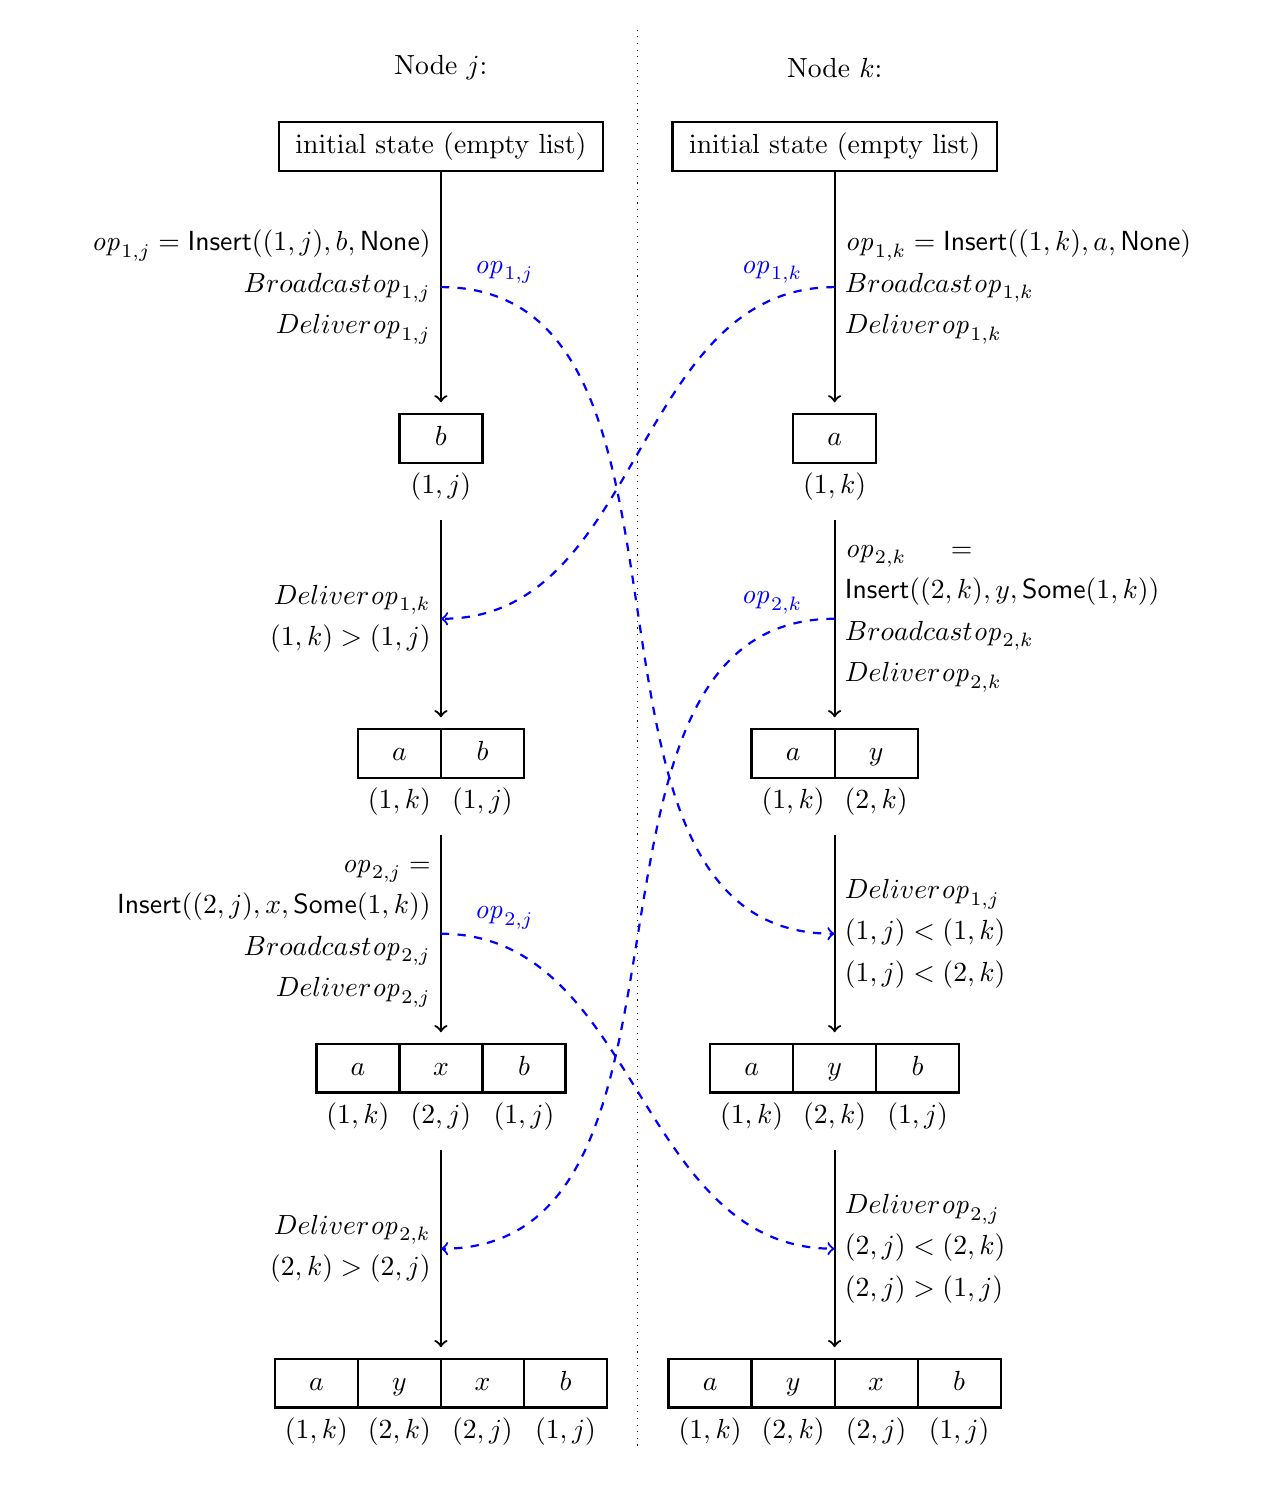
\begin{tikzpicture}[auto,scale=1.0]
\onehalfspacing
\path [draw,dotted] (2.5,-0.5) -- (2.5,17.5);

\tikzstyle{initstate}=[rectangle,draw,inner xsep=6pt,text height=8pt,text depth=3pt]
\tikzstyle{state}=[matrix,column sep={30pt,between origins}]
\tikzstyle{val}=[draw,anchor=base,minimum width=30pt,text height=8pt,text depth=3pt]
\tikzstyle{oid}=[anchor=base]
\tikzstyle{leftevent}=[left,text width=5cm,text ragged left,midway]
\tikzstyle{rightevent}=[right,text width=5cm,text ragged,midway]
\tikzstyle{every path}=[thick,->]

\node (leftR) at (0,17) {Node $j$:};
\node (left1) at (0,16) [initstate] {initial state (empty list)};
\node (left2) at (0,12) [state] {
    \node [val] {$b$};     \\
    \node [oid] {$(1,j)$}; \\
};
\node (left3) at (0,8) [state] {
    \node [val] {$a$};     & \node [val] {$b$};     \\
    \node [oid] {$(1,k)$}; & \node [oid] {$(1,j)$}; \\
};
\node (left4) at (0,4) [state] {
    \node [val] {$a$};     & \node [val] {$x$};     & \node [val] {$b$};     \\
    \node [oid] {$(1,k)$}; & \node [oid] {$(2,j)$}; & \node [oid] {$(1,j)$}; \\
};
\node (left5) at (0,0) [state] {
    \node [val] {$a$};     & \node [val] {$y$};     & \node [val] {$x$};     & \node [val] {$b$};     \\
    \node [oid] {$(1,k)$}; & \node [oid] {$(2,k)$}; & \node [oid] {$(2,j)$}; & \node [oid] {$(1,j)$}; \\
};

\draw (left1) -- (left2) node (send1j) [leftevent] {
    \hfill $\mathit{op}_{1,j} = \mathsf{Insert}((1, j), b, \mathsf{None})$ \\
    \hfill $\text{Broadcast } \mathit{op}_{1,j}$ \\
    \hfill $\text{Deliver } \mathit{op}_{1,j}$ \\
};
\draw (left2) -- (left3) node (recv1k) [leftevent] {
    \hfill $\text{Deliver } \mathit{op}_{1,k}$ \\
    \hfill $(1,k) > (1,j)$ \\
};
\draw (left3) -- (left4) node (send2j) [leftevent] {
    \hfill $\mathit{op}_{2,j} = \mathsf{Insert}((2, j), x, \mathsf{Some}(1,k))$ \\
    \hfill $\text{Broadcast } \mathit{op}_{2,j}$ \\
    \hfill $\text{Deliver } \mathit{op}_{2,j}$ \\
};
\draw (left4) -- (left5) node (recv2k) [leftevent] {
    \hfill $\text{Deliver } \mathit{op}_{2,k}$ \\
    \hfill $(2,k) > (2,j)$ \\
};

\node (rightR) at (5,17) {Node $k$:};
\node (right1) at (5,16) [initstate] {initial state (empty list)};
\node (right2) at (5,12) [state] {
    \node [val] {$a$};     \\
    \node [oid] {$(1,k)$}; \\
};
\node (right3) at (5,8) [state] {
    \node [val] {$a$};     & \node [val] {$y$};     \\
    \node [oid] {$(1,k)$}; & \node [oid] {$(2,k)$}; \\
};
\node (right4) at (5,4) [state] {
    \node [val] {$a$};     & \node [val] {$y$};     & \node [val] {$b$};     \\
    \node [oid] {$(1,k)$}; & \node [oid] {$(2,k)$}; & \node [oid] {$(1,j)$}; \\
};
\node (right5) at (5,0) [state] {
    \node [val] {$a$};     & \node [val] {$y$};     & \node [val] {$x$};     & \node [val] {$b$};     \\
    \node [oid] {$(1,k)$}; & \node [oid] {$(2,k)$}; & \node [oid] {$(2,j)$}; & \node [oid] {$(1,j)$}; \\
};

\draw (right1) -- (right2) node (send1k) [rightevent] {
    $\mathit{op}_{1,k} = \mathsf{Insert}((1, k), a, \mathsf{None})$ \\
    $\text{Broadcast } \mathit{op}_{1,k}$ \\
    $\text{Deliver } \mathit{op}_{1,k}$ \\
};
\draw (right2) -- (right3) node (send2k) [rightevent] {
    $\mathit{op}_{2,k} = \mathsf{Insert}((2, k), y, \mathsf{Some}(1, k))$ \\
    $\text{Broadcast } \mathit{op}_{2,k}$ \\
    $\text{Deliver } \mathit{op}_{2,k}$ \\
};
\draw (right3) -- (right4) node (recv1j) [rightevent] {
    $\text{Deliver } \mathit{op}_{1,j}$ \\
    $(1,j) < (1,k)$ \\
    $(1,j) < (2,k)$ \\
};
\draw (right4) -- (right5) node (recv2j) [rightevent] {
    $\text{Deliver } \mathit{op}_{2,j}$ \\
    $(2,j) < (2,k)$ \\
    $(2,j) > (1,j)$ \\
};

\begin{scope}[dashed,blue]
    \tikzstyle{every node}=[text centered]
    \draw (send1j.east) to [out=0,in=180] (recv1j.west);
    \draw (send2j.east) to [out=0,in=180] (recv2j.west);
    \draw (send1k.west) to [out=180,in=0] (recv1k.east);
    \draw (send2k.west) to [out=180,in=0] (recv2k.east);
    \node at (0.8,14.4) {$\mathit{op}_{1,j}$};
    \node at (0.8, 6.2) {$\mathit{op}_{2,j}$};
    \node at (4.2,14.4) {$\mathit{op}_{1,k}$};
    \node at (4.2,10.2) {$\mathit{op}_{2,k}$};
\end{scope}
\end{tikzpicture}

\caption{RGA example}\label{fig.two-lists}
\end{figure}

\section{Related Work}\label{sect.relatedwork}

In a system where different replicas may concurrently perform updates without coordinating with each
other, strong eventual consistency (SEC, see Section~\ref{sect.eventual.consistency}) requires a
conflict resolution algorithm to reconcile concurrent updates. In some cases, a trivial algorithm is
used, for example:

\begin{description}
\item[User-defined conflict resolution:] Some systems store all conflicting versions of the data,
and either leave it for manual resolution by a user, or invoke a user-defined merge function.
However, manual resolution is an unacceptable burden for the user in many applications, and defining
merge functions in application code is error-prone; for example, \citet{DeCandia:2007ui} describe a
shopping cart anomaly at Amazon that arose due to poor conflict resolution.

\item[Last write wins (LWW):] Each version of the data structure is assigned a unique timestamp.
When there is a conflict, the system picks the version with the highest timestamp and discards other
versions. Although LWW achieves convergence, it does so at the cost of losing user input, which is
often unacceptable.
\end{description}

However, there are also algorithms that achieve convergence automatically, without discarding
updates. In Sections~\ref{sect.related.crdts} and~\ref{sect.related.ot} we summarise two main lines
of work, CRDTs and OT, which have the same fundamental goal of conflict resolution and convergence,
but which take different approaches towards achieving it.

\subsection{Conflict-Free Replicated Data Types (CRDTs)}\label{sect.related.crdts}

Some operations, such as addition of numbers, are naturally commutative. Thus, if the replicated
data structure is a number whose value can only be incremented or decremented (a counter),
convergence can be achieved by applying the increment and decrement operations in any order at each
replica.

\emph{Conflict-free replicated data types} (CRDTs) generalise this idea to other data structures and
operations. For example, an ordered list (sequence) of values can be modified by inserting or
deleting elements at specified positions, and a map (dictionary) datatype can be modified by setting
the value associated with a key or deleting a key-value pair from the map. In a CRDT, those
modification operations are constructed to be commutative by attaching additional metadata to the
data structure.

To propagate changes between replicas, a CRDT either captures every update as an operation and
broadcasts it to other replicas (an \emph{operation-based} CRDT), or periodically broadcasts its
entire replica state (a \emph{state-based} CRDT). Operation-based CRDTs require operations to be
commutative; state-based CRDTs require a merge function over a join-semilattice, allowing two states
to be combined such that the result reflects changes made in both replicas. The two models have
different performance characteristics, but equivalent expressivity
\cite{Shapiro:2011wy,Shapiro:2011un}.

Many common abstract datatypes have been formulated as CRDTs, including
registers \cite{Shapiro:2011wy,Shapiro:2011un}, counters, maps \cite{Baquero:2016iv},
sets \cite{Bieniusa:2012wu,Bieniusa:2012gt}, XML \cite{Martin:2010ih},
and JSON trees \cite{Kleppmann:2016ve}. For ordered lists, several algorithms have been defined:
RGA \cite{Roh:2011dw}, Treedoc \cite{Preguica:2009fz}, WOOT \cite{Oster:2006wj},
Logoot \cite{Weiss:2010hx}, and LSEQ \cite{Nedelec:2013ky,Nedelec:2016eo}.
State-based CRDTs have been deployed commercially in the Riak database \cite{Brown:2014hs}.
Cloud types \cite{Burckhardt:2012jy} have similarities to CRDTs, using a relational data model.

In this work we formally verify three representative operation-based CRDTs: a counter
\cite{Shapiro:2011wy}, an OR-Set \cite{Bieniusa:2012gt}, and the RGA algorithm for ordered lists
\cite{Roh:2011dw}. While the counter and set are quite straightforward, RGA is subtle; we first
describe it informally in Section~\ref{sect.rga.background}, before showing how to formally prove
its convergence.


\subsection{Operational Transformation (OT)}\label{sect.related.ot}

Another family of algorithms for achieving convergence of replicas uses the \emph{operational
transformation} (OT) approach. They are designed for collaborative editing, that is, multiple users
concurrently modifying a document on their local device, and propagating updates asynchronously to
other users' devices. The replicated data structure is most commonly assumed to be a text document,
represented as an ordered list of characters that may be modified by inserting or deleting
characters at arbitrary positions in the string. OT algorithms for ordered lists include
dOPT \cite{Ellis:1989ue}, Jupiter \cite{Nichols:1995fd}, adOPTed \cite{Ressel:1996wx},
GOT \cite{Sun:1998un}, GOTO \cite{Sun:1998vf}, SOCT2 \cite{Suleiman:1997gl,Suleiman:1998eu},
SOCT3/4 \cite{Vidot:2000ch}, IMOR \cite{Imine:2003ks}, SDT \cite{Li:2004er,Li:2008hw}, and
TTF \cite{Oster:2006tr}.  The approach has also been generalised to other data structures such as
XML trees \cite{Ignat:2003jy,Davis:2002iv,Jungnickel:2015ua} and vector graphics documents
\cite{Sun:2002jb}.

Unlike CRDTs, in which update operations are commutative by definition, OT allows non-commutative
operations. Instead, OT relies on \emph{transforming} concurrent operations, allowing them to be
reordered on different nodes while ensuring a convergent outcome.

The required properties of this transformation function depend on assumptions about the network.
Many OT algorithms assume that operations are sequenced through a central server and delivered to
all clients in the same order. This design was originally pioneered by the Jupiter system
\cite{Nichols:1995fd} and is now used by all widely-deployed OT-based collaboration systems,
including Google Docs \cite{DayRichter:2010tt}, Microsoft Word Online, Etherpad
\cite{Etherpad:2011um}, Apache (formerly Google) Wave \cite{Wang:2015vo}, and Novell Vibe
\cite{Spiewak:2010vw}. With a central server, each client only needs to reorder its operations with
respect to the server's operation sequence, which simplifies the transformation.

On the other hand, as discussed in Section~\ref{sect.background.networks}, total order broadcast is
too restrictive for many peer-to-peer systems. Without total order broadcast, OT algorithms must
tolerate a higher degree of concurrency. Although a number of OT algorithms were purported to
guarantee convergence in peer-to-peer networks, many of them were later proved to be incorrect, as
discussed in the next section.

\subsection{Formal Verification}\label{sect.related.verification}

Even though a data structure such as an ordered list may seem as though it ought to be simple, the
history of algorithms for achieving convergence in a distributed setting has been fraught with
difficulty. Informal reasoning has repeatedly produced approaches that fail to converge in certain
scenarios, and even several formal ``proofs'' later turned out to be false.

For OT, the properties that the transformation function must satisfy were first formalised by
\citet{Ressel:1996wx}. These properties are known as $\mathit{TP}_1$ and $\mathit{TP}_2$; systems
with a central server or total order broadcast need only satisfy $\mathit{TP}_1$, whereas
decentralised systems must satisfy both properties in order to ensure convergence. While
$\mathit{TP}_1$ has proved to be readily achievable in practice, and all the aforementioned
widely-deployed OT systems rely on it, the $\mathit{TP}_2$ property has been a significant source of
problems.

The original peer-reviewed publications of dOPT, adOPTed, IMOR, SOCT2, and SDT all claimed that
their transformation functions satisfied $\mathit{TP}_2$, but those claims were subsequently shown
to be false by giving counter-examples \cite{Imine:2003ks,Imine:2006kn,Oster:2005vi}. In the case of
dOPT and adOPTed, the $\mathit{TP}_2$ claim had originally been asserted without proof. In the case
of SOCT2 and SDT, there were hand-written ``proofs'' that later turned out to be incorrect. For IMOR
and SOCT2, there had even been machine-checked ``proofs'' \cite{Imine:2003ks}, but
\citet{Oster:2005vi} showed that they also were invalid because they made incorrect assumptions.

\citet{Randolph:2015gj} have even shown that in the classic formulation of OT it is impossible to
achieve $\mathit{TP}_2$. To our knowledge, TTF is at present the only $\mathit{TP}_2$-claiming OT
algorithm for which no counter-example is known, and it circumvents the impossibility result of
\citet{Randolph:2015gj} by using a different formulation of the transformation
\cite{Oster:2006tr,Levien:2016wz}.

Formal proofs of the $\mathit{TP}_1$ property have been more successful: \citet{Sinchuk:2016cf} and
\citet{Jungnickel:2015ua} verify transformation functions for trees, using Coq and Isabelle/HOL
respectively. For CRDTs, the only machine-checked verification of which we are aware is an Isabelle
formalisation of state-based sets, registers, and counters by \citet{Zeller:2014fl}; this work does
not consider any ordered list datatypes or any operation-based CRDTs.

The convergence of the RGA CRDT for ordered lists, which we study in this paper, has previously been
demonstrated in handwritten proofs \cite{Attiya:2016kh,Kleppmann:2016ve,Roh:2009ws}. Although we
have no reason to doubt the correctness of those proofs, the historic experience with
$\mathit{TP}_2$ makes us wary of claims whose assumptions and reasoning process have not been
checked rigorously. Other authors have also pointed out that handwritten proofs are laborious and
difficult to check by hand \cite{Li:2008hw,Li:2005jq}.

To our knowledge, our work is the first mechanised proof of operation-based CRDTs in general, and of
any ordered list CRDT in particular. As \citet{Oster:2005vi} have demonstrated, machine-checked
proofs are not immune to errors that are due to false assumptions. To avoid this trap, we prove not
only the commutativity of operations (which is subject to certain assumptions), but also that those
assumptions are guaranteed to hold in all executions of our network model. The network model in turn
is specified by a small set of axioms that are not specific to any particular CRDT, and whose
correctness can be robustly defended (see Section~\ref{sect.network}).

\citet{Burckhardt:2014ft} present a similar framework for reasoning about replicated datatypes, but
do not support mechanised proofs at present.


\section{The Replicated Growable Array (RGA)}\label{sect.rga.background}

In order to develop an intuition for the problems that arise in concurrent editing systems, we now
discuss an example execution of the \emph{Replicated Growable Array} (RGA) algorithm, a CRDT for
ordered lists that supports insertion and deletion of arbitrary elements. RGA was developed by
\citet{Roh:2011dw}, although our presentation of the algorithm more closely follows that of
\citet{Shapiro:2011wy}. We start with the informal example illustrated in
Figure~\ref{fig.two-lists}, and leave the formal specification of RGA until Section~\ref{sect.rga}.

In this paper we
choose to analyze RGA because it is a subtle algorithm that benefits from formal verification
\cite{Attiya:2016kh}, because it has been shown to have good performance \cite{Mehdi:2011ke}, and
because it has been generalised to more general data structures such as JSON
\cite{Kleppmann:2016ve}, enabling our work to be extended towards those more general data structures
in future.

RGA is based on the idea of assigning a unique identifier (ID) to each list element, and using a
total ordering relation over IDs to ensure convergence. When the list is modified through insertion
and deletion operations, the ID of an existing element is used to identify the position in the list
being modified. Using an ID has the advantage that it continues to refer to the same list element
regardless of any concurrent operations, whereas list indexes change (for example, inserting a list
element at the beginning increases the index of every subsequent list element by 1).

We use the logical timestamps defined by \citet{Lamport:1978jq} as IDs.

% In this setting, causally ordered delivery is the strongest
% guarantee that can reliably be provided \cite{Attiya:2015dm}.

% \subsubsection{Causal Ordering}
\subsection{Causality and the Happens-Before Relation}\label{sect.causality}

Most operation-based CRDTs and OT algorithms require that operations are processed in an order that
is \emph{consistent with causality}. Informally, this means that later operations may depend on
earlier operations; for example, the deletion of a list element depends on the prior insertion of
that list element. It makes no sense for a replica to apply the deletion before it applies the
insertion, because that would mean deleting an element that does not yet exist at that time.

In this context, referring to operations as ``earlier'' or ``later'' does not mean comparing the
physical time in UTC at which those operations occurred; relying on physical time is often
problematic in distributed systems \cite{Sheehy:2015jm}. Instead we say that an operation
$\mathit{op}_1$ \emph{happens before} another operation $\mathit{op}_2$ if the node that generated
$\mathit{op}_2$ ``knew about'' $\mathit{op}_1$ at the time $\mathit{op}_2$ was generated (i.e., if
$\mathit{op}_1$ had already been applied at that time). If the node knew about $\mathit{op}_1$, then
$\mathit{op}_2$ may somehow be caused by it, but if it didn't know about $\mathit{op}_1$, we can be
certain that $\mathit{op}_2$ does not depend on it.

We write $\mathit{op}_1 \prec \mathit{op}_2$ if $\mathit{op}_1$ happens before $\mathit{op}_2$. (In
the distributed systems literature, the happens-before relation is usually written
$\mathit{op}_1 \longrightarrow \mathit{op}_2$, but we reserve the arrow to refer to logical
implication.) Following the definition by \citet{Lamport:1978jq}, we say that
$\mathit{op}_1 \prec \mathit{op}_2$ if any of the following is true:

\begin{itemize}
\item $\mathit{op}_1$ and $\mathit{op}_2$ were generated by the same node, and that node generated
    $\mathit{op}_1$ before it generated $\mathit{op}_2$.
\item The node that generated $\mathit{op}_2$ had received and applied $\mathit{op}_1$ before it
    generated $\mathit{op}_2$.
\item There exists some operation $\mathit{op}_3$ such that
    $\mathit{op}_1 \prec \mathit{op}_3$ and $\mathit{op}_3 \prec \mathit{op}_2$.
\end{itemize}

\begin{figure}
\centering
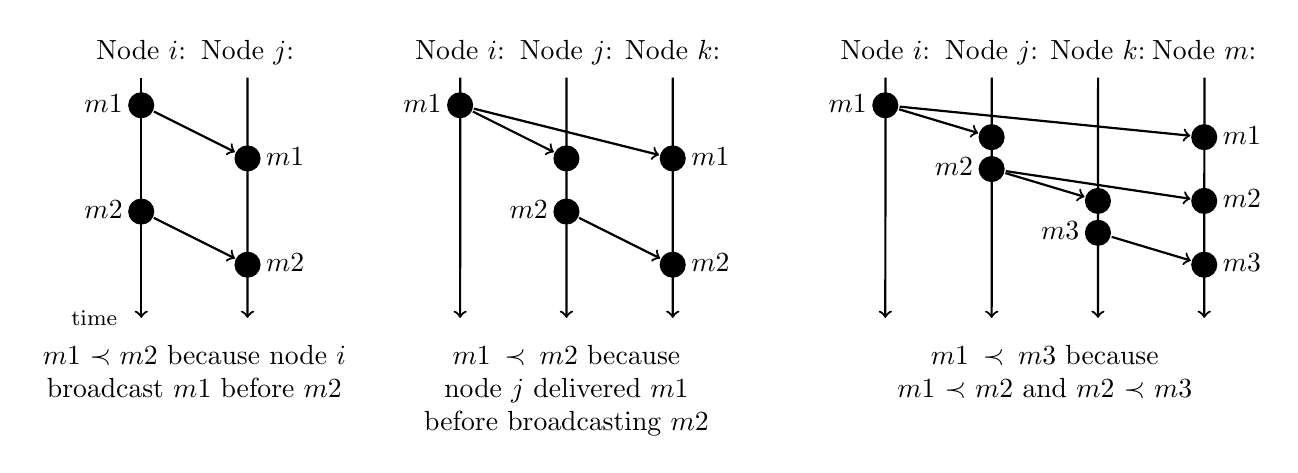
\begin{tikzpicture}[auto,scale=1.35]

\tikzstyle{event}=[circle,fill,minimum size=2pt]
\tikzstyle{label}=[text height=8pt,text depth=3pt]
\tikzstyle{leftlabel}=[label,left=3pt]
\tikzstyle{rightlabel}=[label,right=3pt]
\tikzstyle{every path}=[thick,->]
\tikzstyle{caption}=[text width=4cm,text centered,text height=8pt,below=5pt]

\node [label] (i1name) at (0,2.5) {Node $i$:};
\node [label] (j1name) at (1,2.5) {Node $j$:};
\node [event] (op1send) at (0,2.0) {};
\node [event] (op1recv) at (1,1.5) {};
\node [event] (op2send) at (0,1.0) {};
\node [event] (op2recv) at (1,0.5) {};
\node [leftlabel]  at (0,2.0) {$\isa{m1}$};
\node [rightlabel] at (1,1.5) {$\isa{m1}$};
\node [leftlabel]  at (0,1.0) {$\isa{m2}$};
\node [rightlabel] at (1,0.5) {$\isa{m2}$};
\draw (i1name) -- (0,0) node [left=5pt,at end] {\footnotesize time};
\draw (j1name) -- (1,0);
\draw (op1send) -- (op1recv);
\draw (op2send) -- (op2recv);
\node [caption] at (0.5,0) {
    $\isa{m1} \prec \isa{m2}$
    because node $i$ broadcast $\isa{m1}$ before $\isa{m2}$
};

\node [label] (i2name) at (3,2.5) {Node $i$:};
\node [label] (j2name) at (4,2.5) {Node $j$:};
\node [label] (k2name) at (5,2.5) {Node $k$:};
\node [event] (op3send) at (3,2.0) {};
\node [event] (op3recj) at (4,1.5) {};
\node [event] (op3reck) at (5,1.5) {};
\node [event] (op4send) at (4,1.0) {};
\node [event] (op4reck) at (5,0.5) {};
\node [leftlabel]  at (3,2.0) {$\isa{m1}$};
\node [rightlabel] at (5,1.5) {$\isa{m1}$};
\node [leftlabel]  at (4,1.0) {$\isa{m2}$};
\node [rightlabel] at (5,0.5) {$\isa{m2}$};
\draw (i2name) -- (3,0);
\draw (j2name) -- (4,0);
\draw (k2name) -- (5,0);
\draw (op3send) -- (op3recj);
\draw (op3send) -- (op3reck);
\draw (op4send) -- (op4reck);
\node [caption] at (4.0,0) {
    $\isa{m1} \prec \isa{m2}$
    because node $j$ delivered $\isa{m1}$ before broadcasting $\isa{m2}$
};

\node [label] (i3name) at  (7,2.5) {Node $i$:};
\node [label] (j3name) at  (8,2.5) {Node $j$:};
\node [label] (k3name) at  (9,2.5) {Node $k$:};
\node [label] (m3name) at (10,2.5) {Node $m$:};
\node [event] (op5send) at  (7,2.0) {};
\node [event] (op5recj) at  (8,1.7) {};
\node [event] (op5recm) at (10,1.7) {};
\node [event] (op6send) at  (8,1.4) {};
\node [event] (op6reck) at  (9,1.1) {};
\node [event] (op6recm) at (10,1.1) {};
\node [event] (op7send) at  (9,0.8) {};
\node [event] (op7recm) at (10,0.5) {};
\node [leftlabel]  at  (7,2.0) {$\isa{m1}$};
\node [rightlabel] at (10,1.7) {$\isa{m1}$};
\node [leftlabel]  at  (8,1.4) {$\isa{m2}$};
\node [rightlabel] at (10,1.1) {$\isa{m2}$};
\node [leftlabel]  at  (9,0.8) {$\isa{m3}$};
\node [rightlabel] at (10,0.5) {$\isa{m3}$};
\draw (i3name) -- (7,0);
\draw (j3name) -- (8,0);
\draw (k3name) -- (9,0);
\draw (m3name) -- (10,0);
\draw (op5send) -- (op5recj);
\draw (op5send) -- (op5recm);
\draw (op6send) -- (op6reck);
\draw (op6send) -- (op6recm);
\draw (op7send) -- (op7recm);
\node [caption] at (8.5,0) {
    $\isa{m1} \prec \isa{m3}$ because
    $\isa{m1} \prec \isa{m2}$ and
    $\isa{m2} \prec \isa{m3}$
};

\end{tikzpicture}

\caption{Illustrating the happens-before relation}\label{fig.happens-before}
\end{figure}

Figure~\ref{fig.happens-before} illustrates these three cases, and the formalisation of this
definition appears in Section~\ref{sect.network}.

In practice, the happens-before relationship can be captured using vector timestamps
\cite{Schwarz:1994gl,Fidge:1988tv,Raynal:1996jl}, which are used to implement protocols for causally
ordered delivery \cite{Cachin:2011wt}. As these protocols are widely known and well understood, we
leave them out of scope for this paper.


% Total order broadcast ensures that when nodes broadcast a set of messages to other nodes on the
% network, they are delivered in the same order to all recipients. By contrast, causal ordering is a
% weaker guarantee that allows greater concurrency and thus greater nondeterminism in the network.
% However, it has the advantage that it makes no assumptions about the number of nodes that are
% online.

% TODO happens-before


% There are two families of algorithms for collaborative editing: \emph{operational transformation}
% (OT)~\cite{Ellis:1989ue,Ressel:1996wx,Oster:2006tr,Sun:1998vf,Sun:1998un,Suleiman:1998eu,Nichols:1995fd}
% and \emph{conflict-free replicated datatypes}
% (CRDTs)~\cite{Shapiro:2011wy,Roh:2011dw,Preguica:2009fz,Oster:2006wj,Weiss:2010hx,Nedelec:2013ky,Kleppmann:2016ve}.
% Both allow a document to be modified concurrently on different replicas, with changes applied
% immediately to the local copy, while asynchronously propagating changes to other replicas. The
% goal of these algorithms is to ensure that for all concurrent executions, the replicas converge
% toward the same state without any edits being lost, a property known as \emph{strong eventual
% consistency}~\cite{Shapiro:2011un}.


% CRDTs are a more recent development~\cite{Shapiro:2011un}. While OT is based on transforming
% non-commutative operations so that they have the same effect when reordered, CRDTs define operations
% in a way that makes them commutative by design, making them more amenable to peer-to-peer settings
% in which each node may apply edits in a different order. CRDTs also have attractive performance
% characteristics~\cite{Mehdi:2011ke}.

% TODO Various decentralised algorithms have been proposed and all but one (Oster 2006) have
% subsequently been shown to be incorrect.

\begin{figure}
\centering
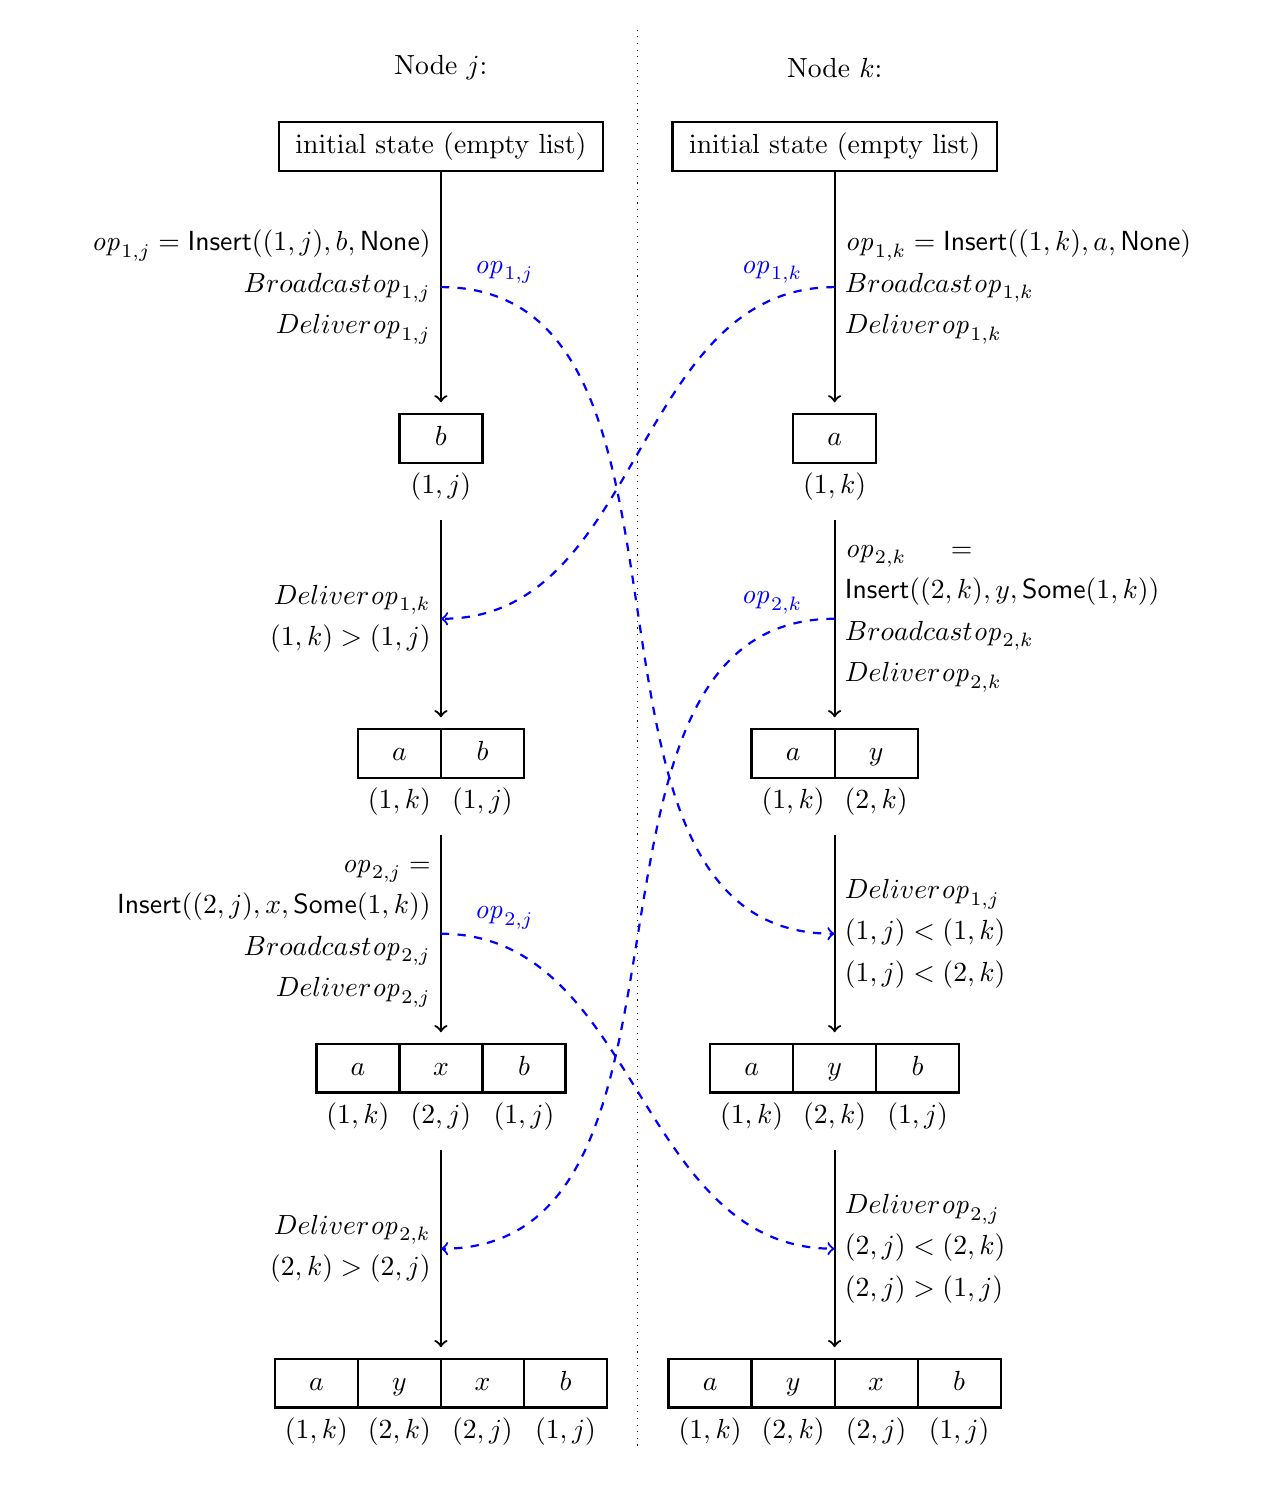
\begin{tikzpicture}[auto,scale=1.0]
\onehalfspacing
\path [draw,dotted] (2.5,-0.5) -- (2.5,17.5);

\tikzstyle{initstate}=[rectangle,draw,inner xsep=6pt,text height=8pt,text depth=3pt]
\tikzstyle{state}=[matrix,column sep={30pt,between origins}]
\tikzstyle{val}=[draw,anchor=base,minimum width=30pt,text height=8pt,text depth=3pt]
\tikzstyle{oid}=[anchor=base]
\tikzstyle{leftevent}=[left,text width=5cm,text ragged left,midway]
\tikzstyle{rightevent}=[right,text width=5cm,text ragged,midway]
\tikzstyle{every path}=[thick,->]

\node (leftR) at (0,17) {Node $j$:};
\node (left1) at (0,16) [initstate] {initial state (empty list)};
\node (left2) at (0,12) [state] {
    \node [val] {$b$};     \\
    \node [oid] {$(1,j)$}; \\
};
\node (left3) at (0,8) [state] {
    \node [val] {$a$};     & \node [val] {$b$};     \\
    \node [oid] {$(1,k)$}; & \node [oid] {$(1,j)$}; \\
};
\node (left4) at (0,4) [state] {
    \node [val] {$a$};     & \node [val] {$x$};     & \node [val] {$b$};     \\
    \node [oid] {$(1,k)$}; & \node [oid] {$(2,j)$}; & \node [oid] {$(1,j)$}; \\
};
\node (left5) at (0,0) [state] {
    \node [val] {$a$};     & \node [val] {$y$};     & \node [val] {$x$};     & \node [val] {$b$};     \\
    \node [oid] {$(1,k)$}; & \node [oid] {$(2,k)$}; & \node [oid] {$(2,j)$}; & \node [oid] {$(1,j)$}; \\
};

\draw (left1) -- (left2) node (send1j) [leftevent] {
    \hfill $\mathit{op}_{1,j} = \mathsf{Insert}((1, j), b, \mathsf{None})$ \\
    \hfill $\text{Broadcast } \mathit{op}_{1,j}$ \\
    \hfill $\text{Deliver } \mathit{op}_{1,j}$ \\
};
\draw (left2) -- (left3) node (recv1k) [leftevent] {
    \hfill $\text{Deliver } \mathit{op}_{1,k}$ \\
    \hfill $(1,k) > (1,j)$ \\
};
\draw (left3) -- (left4) node (send2j) [leftevent] {
    \hfill $\mathit{op}_{2,j} = \mathsf{Insert}((2, j), x, \mathsf{Some}(1,k))$ \\
    \hfill $\text{Broadcast } \mathit{op}_{2,j}$ \\
    \hfill $\text{Deliver } \mathit{op}_{2,j}$ \\
};
\draw (left4) -- (left5) node (recv2k) [leftevent] {
    \hfill $\text{Deliver } \mathit{op}_{2,k}$ \\
    \hfill $(2,k) > (2,j)$ \\
};

\node (rightR) at (5,17) {Node $k$:};
\node (right1) at (5,16) [initstate] {initial state (empty list)};
\node (right2) at (5,12) [state] {
    \node [val] {$a$};     \\
    \node [oid] {$(1,k)$}; \\
};
\node (right3) at (5,8) [state] {
    \node [val] {$a$};     & \node [val] {$y$};     \\
    \node [oid] {$(1,k)$}; & \node [oid] {$(2,k)$}; \\
};
\node (right4) at (5,4) [state] {
    \node [val] {$a$};     & \node [val] {$y$};     & \node [val] {$b$};     \\
    \node [oid] {$(1,k)$}; & \node [oid] {$(2,k)$}; & \node [oid] {$(1,j)$}; \\
};
\node (right5) at (5,0) [state] {
    \node [val] {$a$};     & \node [val] {$y$};     & \node [val] {$x$};     & \node [val] {$b$};     \\
    \node [oid] {$(1,k)$}; & \node [oid] {$(2,k)$}; & \node [oid] {$(2,j)$}; & \node [oid] {$(1,j)$}; \\
};

\draw (right1) -- (right2) node (send1k) [rightevent] {
    $\mathit{op}_{1,k} = \mathsf{Insert}((1, k), a, \mathsf{None})$ \\
    $\text{Broadcast } \mathit{op}_{1,k}$ \\
    $\text{Deliver } \mathit{op}_{1,k}$ \\
};
\draw (right2) -- (right3) node (send2k) [rightevent] {
    $\mathit{op}_{2,k} = \mathsf{Insert}((2, k), y, \mathsf{Some}(1, k))$ \\
    $\text{Broadcast } \mathit{op}_{2,k}$ \\
    $\text{Deliver } \mathit{op}_{2,k}$ \\
};
\draw (right3) -- (right4) node (recv1j) [rightevent] {
    $\text{Deliver } \mathit{op}_{1,j}$ \\
    $(1,j) < (1,k)$ \\
    $(1,j) < (2,k)$ \\
};
\draw (right4) -- (right5) node (recv2j) [rightevent] {
    $\text{Deliver } \mathit{op}_{2,j}$ \\
    $(2,j) < (2,k)$ \\
    $(2,j) > (1,j)$ \\
};

\begin{scope}[dashed,blue]
    \tikzstyle{every node}=[text centered]
    \draw (send1j.east) to [out=0,in=180] (recv1j.west);
    \draw (send2j.east) to [out=0,in=180] (recv2j.west);
    \draw (send1k.west) to [out=180,in=0] (recv1k.east);
    \draw (send2k.west) to [out=180,in=0] (recv2k.east);
    \node at (0.8,14.4) {$\mathit{op}_{1,j}$};
    \node at (0.8, 6.2) {$\mathit{op}_{2,j}$};
    \node at (4.2,14.4) {$\mathit{op}_{1,k}$};
    \node at (4.2,10.2) {$\mathit{op}_{2,k}$};
\end{scope}
\end{tikzpicture}

\caption{RGA example}\label{fig.two-lists}
\end{figure}

\section{An Introduction to Isabelle}
\label{subsect.an.overview.of.isabelle}

We now provide a brief introduction to the key concepts and syntax of Isabelle/HOL.
Familiar readers may skip to Section~\ref{sect.abstract.convergence}.
A more detailed introduction can be found in the standard tutorial material~\cite{DBLP:books/sp/NipkowK14}.

\paragraph{Syntax of expressions.}

Isabelle/HOL is a logic with a strict, polymorphic, inferred type system.
\emph{Function types} are written $\tau_1 \Rightarrow \tau_2$, and are inhabited by \emph{total} functions, mapping elements of $\tau_1$ to elements of $\tau_2$.
We write $\tau_1 \times \tau_2$ for the \emph{product type} of $\tau_1$ and $\tau_2$, inhabited by pairs of elements of type $\tau_1$ and $\tau_2$, respectively.
In a similar fashion to Standard ML and OCaml, \emph{type operators} are applied to arguments in reverse order, and therefore $\tau\ \isa{list}$ denotes the type of lists of elements of type $\tau$, and $\tau\ \isa{set}$ denotes the type of mathematical (i.e., potentially infinite) sets of type $\tau$.
Type variables are written in lowercase, and preceded with a prime: ${\isacharprime}a \Rightarrow {\isacharprime}a$ denotes the type of a polymorphic identity function, for example.
\emph{Tagged union} types are introduced with the $\isacommand{datatype}$ keyword, with constructors of these types usually written with an initial upper case letter.

In Isabelle/HOL's term language we write $\isa{t} \mathbin{::} \tau$ for a \emph{type ascription}, constraining the type of the term $\isa{t}$ to the type $\tau$.
We write $\lambda{x}.\: t$ for an anonymous function mapping an argument $\isa{x}$ to $\isa{t(x)}$, and write the application of term $\isa{t}$ with function type to an argument $\isa{u}$ as $\isa{t\ u}$, as usual.
Terms of list type are introduced using one of two constructors: the empty list $[\,]$ or `nil', and the infix operator $\isa{\#}$ which is pronounced ``cons'', and which prepends an element to an existing list.
We use $[t_1, \ldots, t_n]$ as syntactic sugar for a list literal, and $\isa{xs} \mathbin{\isacharat} \isa{ys}$ to express the concatenation (appending) of two lists $\isa{xs}$ and $\isa{ys}$.
We write $\{\,\}$ for the empty set, and use usual mathematical notation for set union, disjunction, membership tests, and so on: $\isa{t} \cup \isa{u}$, $\isa{t} \cap \isa{u}$, and $\isa{x} \in \isa{t}$.
We write $t \longrightarrow s$ for logical implication between formulae (terms of type $\isa{bool}$).
An alternative implication arrow $\isa{t} \Longrightarrow \isa{u}$ is used by Isabelle in certain contexts; it is subtly different from standard implication $\isa{t} \longrightarrow \isa{u}$, but for purposes of an intuitive understanding, the two forms of implication can be regarded as equivalent.

\paragraph{Definitions and theorems.}

New non-recursive definitions are entered into Isabelle's global context using the $\mathbf{definition}$ keyword.
Recursive functions are defined using the $\mathbf{fun}$ keyword, and support pattern matching on their arguments.
All functions are total, and therefore every recursive function must be provably terminating.
The termination proofs in this work are generated automatically by Isabelle itself.

Inductive relations are defined with the $\mathbf{inductive}$ keyword.
For example, the definition
\vspace{0.35em}
\begin{isabellebody}
\ \ \ \ \ \ \ \ \isacommand{inductive} only-fives\ {\isacharcolon}{\isacharcolon}\ {\isachardoublequoteopen}nat\ list\ {\isasymRightarrow}\ bool{\isachardoublequoteclose}\ \isakeyword{where}\isanewline
\ \ \ \ \ \ \ \ \ \ {\isachardoublequoteopen}only-fives\ {\isacharbrackleft}{\isacharbrackright}{\isachardoublequoteclose}\ {\isacharbar}\isanewline
\ \ \ \ \ \ \ \ \ \ {\isachardoublequoteopen}{\isasymlbrakk}\ only-fives\ xs\ {\isasymrbrakk}\ {\isasymLongrightarrow}\ only-fives {\isacharparenleft}5\#xs{\isacharparenright}{\isachardoublequoteclose}
\end{isabellebody}
\vspace{0.35em}
\noindent
introduces a new constant $\isa{only-fives}$ of type $\isa{nat list} \Rightarrow \isa{bool}$.
The two clauses in the body of the definition enumerate the conditions under which $\isa{only-fives}\ \isa{xs}$ is true, for arbitrary $\isa{xs}$: firstly, $\isa{only-fives}$ is true for the empty list; and secondly, if you know that $\isa{only-fives}\ \isa{xs}$ is true for some $\isa{xs}$, then you can deduce that $\isa{only-fives}\ (5\#\isa{xs})$ (i.e., $\isa{xs}$ prefixed with the number 5) is also true.
Moreover, $\isa{only-fives}\ \isa{xs}$ is true in no other circumstances---it is the \emph{smallest} relation closed under the rules defining it.
In short, the clauses above state that $\isa{only-fives}\ \isa{xs}$ holds exactly in the case where $\isa{xs}$ is a (potentially empty) list containing only repeated copies of the natural number $5$.

Lemmas, theorems, and corollaries can be asserted using the $\isacommand{lemma}$, $\isacommand{theorem}$, and $\isacommand{corollary}$ keywords, respectively.
There is no semantic difference between these keywords in Isabelle.
For example,
\vspace{0.35em}
\begin{isabellebody}
\ \ \ \ \ \ \ \ \isacommand{theorem} only-fives-concat{\isacharcolon}\isanewline
\ \ \ \ \ \ \ \ \ \ \isakeyword{assumes}\ only-fives\ xs \isakeyword{and}\ only-fives\ ys \isanewline
\ \ \ \ \ \ \ \ \ \ \isakeyword{shows}\ only-fives (xs \isacharat ys)
\end{isabellebody}
\vspace{0.35em}
\noindent
conjectures that if $\isa{xs}$ and $\isa{ys}$ are both lists of fives, then their concatenation $xs \mathbin{\isacharat} ys$ is also a list of fives.
Isabelle then requires that this claim be proved by using one of its proof methods, for example by induction.
Some proofs can be automated, whilst others require the user to provide explicit reasoning steps.
The theorem is assigned a name, here $\isa{only-fives-concat}$, so that it may be referenced in later proofs.

\paragraph{Locales.}

Lastly, we use \emph{locales}---or local theories~\cite{DBLP:conf/tphol/KammullerWP99,DBLP:conf/types/HaftmannW08}---extensively to structure the proof, as shown in Figure~\ref{fig.proof.structure}.
A declaration of the form
\vspace{0.35em}
\begin{isabellebody}
\ \ \ \ \ \ \ \ \isacommand{locale} semigroup = \isanewline
\ \ \ \ \ \ \ \ \ \ \isakeyword{fixes}\ f\ {\isacharcolon}{\isacharcolon}\ {\isachardoublequoteopen}{\isacharprime}a\ {\isasymRightarrow}\ {\isacharprime}a{\isachardoublequoteclose}\ {\isasymRightarrow}\ {\isacharprime}a{\isachardoublequoteclose} \isanewline
\ \ \ \ \ \ \ \ \ \ \isakeyword{assumes} {\isachardoublequoteopen}f\ x\ (f\ y\ z)\ =\ f\ (f\ x\ y)\ z{\isachardoublequoteclose}
\end{isabellebody}
\vspace{0.35em}
\noindent
introduces a locale, with a fixed, typed constant $\isa{f}$, and a law asserting that $\isa{f}$ is associative.
Functions and constants may now be defined, and theorems conjectured and proved, within the context of the $\isa{semigoup}$ locale.
This is indicated syntactically by writing $(\isacommand{in}\ \isa{semigroup})$ before the name of the constant being defined, or the theorem being conjectured, at the point of definition or conjecture.
Any function, constant, or theorem, marked in this way may make reference to $\isa{f}$, or the fact that $\isa{f}$ is associative.
\emph{Interpreting} a locale---such as $\isa{semigroup}$ above---involves providing a concrete implementation of $\isa{f}$ coupled with a proof that the concrete implementation satisfies the associated law.
Once interpreted, all functions, definitions, and theorems made within the $\isa{semigroup}$ locale become available to use for that concrete implementation.

\section{Abstract convergence}
\label{sect.abstract.convergence}

Strong eventual consistency requires \emph{convergence} of all copies of shared state stored on nodes in the distributed system.
It guarantees that whenever two nodes have received the same set of updates to shared state---possibly in a different order---their view of the shared state is always identical.
This definition constrains the values that read operations may return at any time, making it a stronger property than eventual consistency.
By accessing only their local copy of the shared state, nodes can execute read and write operations without waiting for network communication.
Nodes exchange updates asynchronously when a network connection is available.  

We now use Isabelle to formalise the notion of strong eventual consistency.
In this section we do not make any assumptions about networks, or data structures; instead, we use an abstract model of operations that may be reordered, and we reason about the properties that those operations must satisfy.
We then provide concrete implementations of that abstract model in later sections.

\subsection{The happens-before relation and causality}\label{sect.happens.before}

The simplest way of achieving convergence is to require all operations to be commutative, but this definition is too strong to be useful for many datatypes.
For example, in a list data structure, an element may first be added and then subsequently removed again.
Although it is possible to make such additions and removals unconditionally commutative, doing so yields counterintuitive semantics \cite{Bieniusa:2012wu,Bieniusa:2012gt}.
Instead, a better approach is to require only \emph{concurrent} operations to commute with each other.
Two operations are concurrent if neither ``knew about'' the other at the time when they were generated.
If one operation happened before another---for example, if the removal of an element from a set knew about the prior addition of that element from the set---then it is reasonable to assume that all nodes will apply the operations in that order (first the addition, then the removal).

The \emph{happens-before} relation, as introduced by \citet{Lamport:1978jq}, captures such causal dependencies between operations.
It can be defined in terms of sending and receiving messages on a network, and we give such a definition in Section~\ref{sect.network}.
However, for now, we keep it abstract, writing $\isa{x} \prec \isa{y}$ to indicate that operation $\isa{x}$ happened before $\isa{y}$, where $\prec$ is a predicate of type $\isacharprime\isa{oper} \mathbin{\isasymRightarrow} \isacharprime\isa{oper} \mathbin{\isasymRightarrow} \isa{bool}$.
In words, $\prec$ can be applied to two operations of some abstract type $\isacharprime\isa{oper}$, returning either $\isa{True}$ or $\isa{False}$.%
\footnote{Note that in the distributed systems literature it is conventional to write the happens-before relation as $\isa{x} \rightarrow \isa{y}$, but we reserve the arrow operator to denote logical implication.}
Our only restriction on the happens-before relation $\prec$ is that it must be a \emph{strict partial order}, that is, it must be irreflexive and transitive, which implies that it is also antisymmetric.
We say that two operations $x$ and $y$ are \emph{concurrent}, written $x \mathbin{\isasymparallel} y$, whenever one does not happen before the other:
$\neg (\isa{x} \prec \isa{y})$ and $\neg (\isa{y} \prec \isa{x})$.
Thus, given any two operations $\isa{x}$ and $\isa{y}$, there are three mutually exclusive ways in which they can be related: either $\isa{x} \prec \isa{y}$, or $\isa{y} \prec \isa{x}$, or $\isa{x} \mathbin{\isasymparallel} \isa{y}$.

As discussed above, the purpose of the happens-before relation is to require that some operations must be applied in a particular order, while allowing concurrent operations to be reordered with respect to each other.
We assume that each node applies operations in some sequential order (a standard assumption for distributed algorithms), and so we can model the execution history of a node as a list of operations.
We can then inductively define a list of operations as being \emph{consistent with the happens-before relation}, or simply \emph{hb-consistent}, as follows:
\vspace{0.35em}
\begin{isabellebody}
\ \ \ \ \ \ \ \ \isacommand{inductive} hb{\isacharunderscore}consistent\ {\isacharcolon}{\isacharcolon}\ {\isachardoublequoteopen}{\isacharprime}oper\ list\ {\isasymRightarrow}\ bool{\isachardoublequoteclose}\ \isakeyword{where}\isanewline
\ \ \ \ \ \ \ \ \ \ {\isachardoublequoteopen}hb{\isacharunderscore}consistent\ {\isacharbrackleft}{\isacharbrackright}{\isachardoublequoteclose}\ {\isacharbar}\isanewline
\ \ \ \ \ \ \ \ \ \ {\isachardoublequoteopen}{\isasymlbrakk}\ hb{\isacharunderscore}consistent\ xs{\isacharsemicolon}\ {\isasymforall}x\ {\isasymin}\ set\ xs{\isachardot}\ {\isasymnot}\ y\ {\isasymprec}\ x\ {\isasymrbrakk}\ {\isasymLongrightarrow}\ hb{\isacharunderscore}consistent\ {\isacharparenleft}xs\ {\isacharat}\ {\isacharbrackleft}y{\isacharbrackright}{\isacharparenright}{\isachardoublequoteclose}
\end{isabellebody}
\vspace{0.35em}
In words: the empty list is hb-consistent; furthermore, given an hb-consistent list $\isa{xs}$, we can append an operation $\isa{y}$ to the end of the list to obtain another hb-consistent list, provided that $\isa{y}$ does not happen-before any existing operation $\isa{x}$ in $\isa{xs}$. As a result, whenever two operations $\isa{x}$ and $\isa{y}$ appear in a hb-consistent list, and $\isa{x}\prec\isa{y}$, then $\isa{x}$ must appear before $\isa{y}$ in the list. However, if $\isa{x}\mathbin{\isasymparallel}\isa{y}$, the operations can appear in the list in either order.

\subsection{Interpretation of operations}\label{sect.ops.interpretation}

We describe the state of a node using an abstract type variable $\isacharprime\isa{state}$.
To model state changes, we assume the existence of an \emph{interpretation} function of type $\isa{interp} \mathbin{\isacharcolon\isacharcolon} \isacharprime\isa{oper} \mathbin{\isasymRightarrow} \isacharprime\isa{state} \mathbin{\isasymRightarrow} \isacharprime\isa{state}\ \isa{option}$, which lifts an operation into a \emph{state transformer}---a function that either maps an old state to a new state, or fails by returning $\isa{None}$.
If $\isa{x}$ is an operation, we also write $\langle\isa{x}\rangle$ for the state transformer obtained by applying $\isa{x}$ to the interpretation function.

Concretely, these definitions are captured in Isabelle with the following locale declaration:
\vspace{0.35em}
\begin{isabellebody}
\ \ \ \ \ \ \ \ \isacommand{locale} happens{\isacharunderscore}before\ {\isacharequal}\ preorder\ hb{\isacharunderscore}weak\ hb\isanewline
\ \ \ \ \ \ \ \ \ \ \isakeyword{for}\ hb{\isacharunderscore}weak\ {\isacharcolon}{\isacharcolon}\ {\isachardoublequoteopen}{\isacharprime}oper\ {\isasymRightarrow}\ {\isacharprime}oper\ {\isasymRightarrow}\ bool{\isachardoublequoteclose}\ \ \isakeyword{and}\ hb\ {\isacharcolon}{\isacharcolon}\ {\isachardoublequoteopen}{\isacharprime}oper\ {\isasymRightarrow}\ {\isacharprime}oper\ {\isasymRightarrow}\ bool{\isachardoublequoteclose}\ {\isacharplus}\isanewline
\ \ \ \ \ \ \ \ \ \ \isakeyword{fixes}\ interp\ {\isacharcolon}{\isacharcolon}\ {\isachardoublequoteopen}{\isacharprime}oper\ {\isasymRightarrow}\ {\isacharprime}state\ {\isasymRightarrow}\ {\isacharprime}state\ option{\isachardoublequoteclose}
\end{isabellebody}
\vspace{0.35em}
The $\isa{happens-before}$ locale extends the $\isa{preorder}$ locale, which is part of Isabelle's standard library and includes various useful lemmas.
It fixes two constants: a preorder that we call $\isa{hb-weak}$ or $\preceq$, and a strict partial order that we call $\isa{hb}$ or $\prec$.
We are only interested in the strict partial order, so we define $\isa{hb-weak}$ as $\isa{x}\preceq\isa{y} \equiv \isa{x}\prec\isa{y} \vee \isa{x}=\isa{y}$, and otherwise ignore it.

Moreover, the locale fixes the interpretation function $\isa{interp}$ as described above, which means that we assume the existence of a function with the given type signature without specifying an implementation.
The code in parentheses defines the mixfix operators $\preceq$, $\prec$, and $\langle\isa{x}\rangle$ for notational convenience.

Given two operations $\isa{x}$ and $\isa{y}$, we can now define the composition of state transformers: we write $\langle\isa{x}\rangle \mathbin{\isasymrhd} \langle\isa{y}\rangle$ to denote the state transformer that first applies the effect of $\isa{x}$ to some state, and then applies the effect of $\isa{y}$ to the result.
If either $\langle\isa{x}\rangle$ or $\langle\isa{y}\rangle$ fails, the combined state transformer also fails.
The operator $\isasymrhd$ is a specialised form of the \emph{Kleisli arrow composition}, which we define as:
\vspace{0.35em}
\begin{isabellebody}
\ \ \ \ \ \ \ \ \isacommand{definition} kleisli\ {\isacharcolon}{\isacharcolon}\ {\isachardoublequoteopen}{\isacharparenleft}{\isacharprime}a\ {\isasymRightarrow}\ {\isacharprime}a\ option{\isacharparenright}\ {\isasymRightarrow}\ {\isacharparenleft}{\isacharprime}a\ {\isasymRightarrow}\ {\isacharprime}a\ option{\isacharparenright}\ {\isasymRightarrow}\ {\isacharparenleft}{\isacharprime}a\ {\isasymRightarrow}\ {\isacharprime}a\ option{\isacharparenright}{\isachardoublequoteclose}\ \isakeyword{where}\isanewline
\ \ \ \ \ \ \ \ \ \ {\isachardoublequoteopen}f\ {\isasymrhd}\ g\ {\isasymequiv}\ {\isasymlambda}x{\isachardot}\ f\ x\ {\isasymbind}\ {\isacharparenleft}{\isasymlambda}y{\isachardot}\ g\ y{\isacharparenright}{\isachardoublequoteclose}
\end{isabellebody}
\vspace{0.35em}
Here, $\isasymbind$ is the \emph{monadic bind} operation, defined on the option type that we are using to implement partial functions.
We can now define a function $\isa{apply-operations}$ that composes an arbitrary list of operations into a state transformer.
We first map $\isa{interp}$ across the list to obtain a state transformer for each operation, and then collectively compose them using the Kleisli arrow composition combinator:
\vspace{0.35em}
\begin{isabellebody}
\ \ \ \ \ \ \ \ \isacommand{definition} apply{\isacharunderscore}operations\ {\isacharcolon}{\isacharcolon}\ {\isachardoublequoteopen}{\isacharprime}oper\ list\ {\isasymRightarrow}\ {\isacharprime}state\ {\isasymRightarrow}\ {\isacharprime}state\ option{\isachardoublequoteclose}\ \isakeyword{where}\isanewline
\ \ \ \ \ \ \ \ \ \ {\isachardoublequoteopen}apply{\isacharunderscore}operations\ es\ {\isasymequiv}\ foldl\ {\isacharparenleft}op\ {\isasymrhd}{\isacharparenright}\ Some\ {\isacharparenleft}map\ interp\ es{\isacharparenright}{\isachardoublequoteclose}
\end{isabellebody}
\vspace{0.35em}
The result is a state transformer that applies the interpretation of each of the operations in the list, in left-to-right order, to some initial state.
If any of the operations fails, the entire composition returns $\isa{None}$.

\subsection{Commutativity and convergence}\label{sect.ops.commute}

We say that two operations $\isa{x}$ and $\isa{y}$ \emph{commute} whenever $\langle\isa{x}\rangle \mathbin{\isasymrhd} \langle\isa{y}\rangle = \langle\isa{y}\rangle \mathbin{\isasymrhd} \langle\isa{x}\rangle$, i.e. when we can swap the order of the composition of their interpretations without changing the resulting state transformer.
For our purposes, requiring that this property holds for \emph{all} pairs of operations is too strong.
Rather, the commutation property is only required to hold for operations that are concurrent, as captured in the next definition:
\vspace{0.35em}
\begin{isabellebody}
\ \ \ \ \ \ \ \ \isacommand{definition} concurrent{\isacharunderscore}ops{\isacharunderscore}commute\ {\isacharcolon}{\isacharcolon}\ {\isachardoublequoteopen}{\isacharprime}oper\ list\ {\isasymRightarrow}\ bool{\isachardoublequoteclose}\ \isakeyword{where}\isanewline
\ \ \ \ \ \ \ \ \ \ {\isachardoublequoteopen}concurrent{\isacharunderscore}ops{\isacharunderscore}commute\ xs\ {\isasymequiv} {\isasymforall}x\ y{\isachardot}\ {\isacharbraceleft}x{\isacharcomma}\ y{\isacharbraceright}\ {\isasymsubseteq}\ set\ xs\ {\isasymlongrightarrow}\ x\ {\isasymparallel}\ y\ {\isasymlongrightarrow}\ {\isasymlangle}x{\isasymrangle}{\isasymrhd}{\isasymlangle}y{\isasymrangle}\ {\isacharequal}\ {\isasymlangle}y{\isasymrangle}{\isasymrhd}{\isasymlangle}x{\isasymrangle}{\isachardoublequoteclose}
\end{isabellebody}
\vspace{0.35em}
Given this definition, we can now state and prove our main theorem, $\isa{convergence}$.
This theorem states that two hb-consistent lists of distinct operations, which are permutations of each other and in which concurrent operations commute, have the same interpretation:
\vspace{0.35em}
\begin{isabellebody}
\ \ \ \ \ \ \ \ \isacommand{theorem} convergence{\isacharcolon}\isanewline
\ \ \ \ \ \ \ \ \ \ \isakeyword{assumes}\ {\isachardoublequoteopen}set\ xs\ {\isacharequal}\ set\ ys{\isachardoublequoteclose}\ \isakeyword{and}\ {\isachardoublequoteopen}concurrent{\isacharunderscore}ops{\isacharunderscore}commute\ xs{\isachardoublequoteclose}\ \isakeyword{and}\ {\isachardoublequoteopen}concurrent{\isacharunderscore}ops{\isacharunderscore}commute\ ys{\isachardoublequoteclose}\isanewline
\ \ \ \ \ \ \ \ \ \ \ \ \ \ \ \ \isakeyword{and}\ {\isachardoublequoteopen}distinct\ xs{\isachardoublequoteclose}\ \isakeyword{and}\ {\isachardoublequoteopen}distinct\ ys{\isachardoublequoteclose}\ \isakeyword{and}\ {\isachardoublequoteopen}hb{\isacharunderscore}consistent\ xs{\isachardoublequoteclose}\ \isakeyword{and}\ {\isachardoublequoteopen}hb{\isacharunderscore}consistent\ ys{\isachardoublequoteclose}\isanewline
\ \ \ \ \ \ \ \ \ \ \isakeyword{shows}\ {\isachardoublequoteopen}apply{\isacharunderscore}operations\ xs\ {\isacharequal}\ apply{\isacharunderscore}operations\ ys{\isachardoublequoteclose}
\end{isabellebody}
\vspace{0.35em}
\noindent
A fully mechanised proof of this theorem can be found in the supplementary material of this paper.
Although this theorem may seem ``obvious'' at first glance---commutativity allows the operation order to be permuted---it is more subtle than it seems.
The difficulty arises because operations may succeed when applied to some state, but fail when applied to another state (for example, deleting an element that does not exist in the state).
We find it interesting that it is nevertheless sufficient for the definition of $\isa{concurrent-ops-commute}$ to be expressed only in terms of the Kleisli arrow composition, and without explicitly referring to the state.

\subsection{Formalising Strong Eventual Consistency}\label{sect.abstract.sec.spec}

Besides convergence, another required property of SEC is \emph{progress}: if a valid operation was issued on one node, then applying that operation on other nodes must also succeed---that is, the execution must not become stuck in an error state.
Although the type signature of the interpretation function allows operations to fail, we need to prove that in all $\isa{hb-consistent}$ network behaviours such failure never actually occurs.
We capture the combined requirements of convergence and progress in the $\isa{strong-eventual-consistency}$ locale, which extends $\isa{happens-before}$:
\vspace{0.35em}
\begin{isabellebody}
\ \ \ \ \ \ \ \ \isacommand{locale}\ strong{\isacharunderscore}eventual{\isacharunderscore}consistency\ {\isacharequal}\ happens{\isacharunderscore}before\ {\isacharplus}\ \isakeyword{fixes}\ op{\isacharunderscore}history\ {\isacharcolon}{\isacharcolon}\ {\isachardoublequoteopen}{\isacharprime}oper\ list\ {\isasymRightarrow}\ bool{\isachardoublequoteclose}\ \isakeyword{and}\ initial{\isacharunderscore}state\ {\isacharcolon}{\isacharcolon}\ {\isachardoublequoteopen}{\isacharprime}state{\isachardoublequoteclose}\isanewline
\ \ \ \ \ \ \ \ \ \ \isakeyword{assumes}\ causality{\isacharcolon}\ {\isasymlbrakk}\ {\isachardoublequoteopen}op{\isacharunderscore}history\ xs\ {\isasymrbrakk}\ {\isasymLongrightarrow}\ hb{\isacharunderscore}consistent\ xs{\isachardoublequoteclose}\isanewline
\ \ \ \ \ \ \ \ \ \ \ \ \ \ \isakeyword{and}\ distinctness{\isacharcolon}\ {\isasymlbrakk}\ {\isachardoublequoteopen}op{\isacharunderscore}history\ xs\ {\isasymrbrakk}\ {\isasymLongrightarrow}\ distinct\ xs{\isachardoublequoteclose}\isanewline
\ \ \ \ \ \ \ \ \ \ \ \ \ \ \isakeyword{and}\ trunc{\isacharunderscore}history{\isacharcolon}\ {\isasymlbrakk}\ {\isachardoublequoteopen}op{\isacharunderscore}history{\isacharparenleft}xs{\isacharat}{\isacharbrackleft}x{\isacharbrackright}{\isacharparenright}\ {\isasymrbrakk}\ {\isasymLongrightarrow}\ op{\isacharunderscore}history\ xs{\isachardoublequoteclose}\isanewline
\ \ \ \ \ \ \ \ \ \ \ \ \ \ \isakeyword{and}\ commutativity{\isacharcolon}\ {\isasymlbrakk}\ {\isachardoublequoteopen}op{\isacharunderscore}history\ xs\ {\isasymrbrakk}\ {\isasymLongrightarrow}\ concurrent{\isacharunderscore}ops{\isacharunderscore}commute\ xs{\isachardoublequoteclose}\isanewline
  \ \ \ \ \ \ \ \ \ \ \ \ \ \ \isakeyword{and}\ no{\isacharunderscore}failure{\isacharcolon}\ {\isasymlbrakk}\ {\isachardoublequoteopen}op{\isacharunderscore}history{\isacharparenleft}xs{\isacharat}{\isacharbrackleft}x{\isacharbrackright}{\isacharparenright};\ apply{\isacharunderscore}operations\ xs\ initial{\isacharunderscore}state\ {\isacharequal}\ Some\ state\ {\isasymrbrakk}\ {\isasymLongrightarrow}\ {\isasymlangle}x{\isasymrangle}\ state\ {\isasymnoteq}\ None{\isachardoublequoteclose}
\end{isabellebody}
\vspace{0.35em}
Here, $\isa{op-history}$ is an abstract predicate describing any valid operation history of some replication algorithm.
This locale serves as a concise summary of the properties that we require in order to achieve SEC, and from these assumptions and the theorem above we easily obtain the two safety properties of SEC as theorems:
\vspace{0.35em}
\begin{isabellebody}
\ \ \ \ \ \ \ \ \isacommand{theorem}\ sec{\isacharunderscore}convergence{\isacharcolon}\isanewline
\ \ \ \ \ \ \ \ \ \ \isakeyword{assumes}\ {\isachardoublequoteopen}set\ xs\ {\isacharequal}\ set\ ys{\isachardoublequoteclose}\ \isakeyword{and}\ {\isachardoublequoteopen}op{\isacharunderscore}history\ xs{\isachardoublequoteclose}\ \isakeyword{and}\ {\isachardoublequoteopen}op{\isacharunderscore}history\ ys{\isachardoublequoteclose}\isanewline
\ \ \ \ \ \ \ \ \ \ \isakeyword{shows}\ \ \ {\isachardoublequoteopen}apply{\isacharunderscore}operations\ xs\ {\isacharequal}\ apply{\isacharunderscore}operations\ ys{\isachardoublequoteclose}
\end{isabellebody}
\vspace{0.35em}
\begin{isabellebody}
\ \ \ \ \ \ \ \ \isacommand{theorem}\ sec{\isacharunderscore}progress{\isacharcolon}\isanewline
\ \ \ \ \ \ \ \ \ \ \isakeyword{assumes}\ {\isachardoublequoteopen}op{\isacharunderscore}history\ xs{\isachardoublequoteclose}\ \ \ \isakeyword{shows}\ \ {\isachardoublequoteopen}apply{\isacharunderscore}operations\ xs\ initial{\isacharunderscore}state\ {\isasymnoteq}\ None{\isachardoublequoteclose}
\end{isabellebody}
\vspace{0.35em}
Thus, in order to prove SEC for some replication algorithm, we only need to show that the five assumptions of the $\isa{strong-eventual-consistency}$ locale are satisfied.
As we shall see in Section~\ref{sect.network}, the first three assumptions are satisfied by our network model, and do not require any algorithm-specific proofs.
For individual algorithms we only need to prove the $\isa{commutativity}$ and $\isa{no-failure}$ properties, and we show how to do this in Sections~\ref{sect.rga} and~\ref{sect.simple.crdts}.

\section{An Axiomatic Network Model}
\label{sect.network}

In this section we develop a formal definition of an \emph{asynchronous unreliable causal broadcast network}.
We choose this model because it satisfies the causal delivery requirements of many operation-based CRDTs \cite{Almeida:2015fc,Baquero:2014ed}.
Moreover, it is suitable for use in decentralised settings, as motivated in the introduction, since it does not require waiting for communication with a central server or a quorum of nodes.
Stronger consistency models do not have this property \cite{Attiya:2015dm,Davidson:1985hv}.

The \emph{causal} and \emph{broadcast} aspects of the model are explained in Sections~\ref{sect.network.broadcast} and~\ref{sect.network.causal}.
The \emph{asynchronous} aspect means that we make no timing assumptions: messages sent over the network may suffer unbounded delays before they are delivered, nodes may pause their execution for unbounded periods of time, and we require no clock synchronisation.
\emph{Unreliable} means that messages may never arrive at all, and nodes may fail permanently without warning.
Networks are known to exhibit these behaviours in practice \cite{Bailis:2014jx}, and replication algorithms must tolerate such failures.

This model provides a realistic setting in which we can embed various replication algorithms, and prove that they guarantee SEC in all possible behaviours of the network.
But it is also abstract enough to be able to model a wide range of scenarios: for example, if a user makes updates while offline, and the device re-synchronises when it is next online, we can simply model that interaction as very large network delay.
Our network model is defined using only six axioms, all of which are standard assumptions when modelling distributed systems, and which are satisfied by many systems in practice.
All theorems in this paper are derived from those axioms; in particular, we show that the causal delivery abstraction satisfies the strict partial ordering assumption of $\isa{hb-consistent}$ (Section~\ref{sect.happens.before}), allowing us to use the convergence theorem in any locales that extend the network.

\subsection{Modelling a Distributed System}

We model a distributed system as an unbounded number of communicating nodes.
We assume nothing about the communication pattern of nodes---we assume only that each node is uniquely identified by a natural number, and that the flow of execution at each node consists of a finite, totally ordered sequence of execution steps (events).
We call that sequence of events at node $i$ the \emph{history} of that node.
For convenience, we assume that every event or execution step is unique within a node's history; this assumption is standard when modelling distributed systems \cite{Cachin:2011wt} and can easily be implemented by attaching a sequence number, timestamp, or other unique identifier to each event.
This system model can be expressed in Isabelle as follows:
\begin{isabelle}
~~~~\isakeyword{assumes}\ \=\kill
\isacommand{locale} node{\isacharunderscore}histories\ {\isacharequal}\\
~~~~\isakeyword{fixes}\ \>history\ {\isacharcolon}{\isacharcolon}\ {\isachardoublequoteopen}nat\ {\isasymRightarrow}\ {\isacharprime}a\ list{\isachardoublequoteclose}\ \\
~~~~\isakeyword{assumes}\ \>histories{\isacharunderscore}distinct{\isacharcolon}\ {\isachardoublequoteopen}distinct\ {\isacharparenleft}history\ i{\isacharparenright}{\isachardoublequoteclose}
\end{isabelle}
Here, the history of a node $\isa{i}$ is obtained by using a function fixed by the locale, $\isa{history}$.
The history is simply a list of events, and each event is modelled as an abstract type variable---here we use $\isa{{\isacharprime}a}$.
The $\isa{distinct}$ predicate is an Isabelle/HOL library function that asserts that a list contains no duplicate elements.
Note that we make no assumption about the number of nodes in the system, which allows us to model systems in which nodes join and leave the network over time.
A node that does not exist is simply modelled as an empty list of events.

A node's history is finite, and at the end of a node's history we assume that a node has either failed or successfully terminated.
We treat node failure as permanent, and model it by the absence of any further events in its history.
This \emph{crash-stop} abstraction is commonly used by distributed algorithms \cite{Cachin:2011wt}.

In the $\isa{node{\isacharunderscore}histories}$ locale we may write $\isa{x} \sqsubset^\isa{i} \isa{y}$, which means that event $\isa{x}$ \emph{comes before} event $\isa{y}$ in the history of node $\isa{i}$.
More formally, $\isa{x} \sqsubset^\isa{i} \isa{y}$ if and only if there exist lists $\isa{xs}$, $\isa{ys}$, and $\isa{zs}$ such that $\isa{xs}\mathbin{@}[\isa{x}]\mathbin{@}\isa{ys}\mathbin{@}[\isa{y}]\mathbin{@}\isa{zs} = \isa{history\ i}$.

\subsection{An Asynchronous Broadcast Network}\label{sect.network.broadcast}

We now extend the $\isa{node-histories}$ locale by defining how nodes can communicate.
We specialise $\isacharprime\isa{a}$ to be one of two kinds of event: either \emph{broadcast} or \emph{deliver}.
(In the conventional distributed systems terminology, a \emph{deliver} event indicates that a message was received from the network and delivered to the application.)
Each event contains a message of some abstract type $\isacharprime\isa{msg}$:
\begin{isabelle}
\isacommand{datatype} {\isacharprime}msg\ event\ {\isacharequal}\ Broadcast\ {\isacharprime}msg\ {\isacharbar}\ Deliver\ {\isacharprime}msg
\end{isabelle}

Intuitively, a node can be regarded as a deterministic state machine where each state transition corresponds to a broadcast or deliver event.
We assume that users may query the state of any node at any time, and such queries need not be reflected as events, since they neither modify the node state nor send or receive any messages.

A broadcast abstraction is the standard network model for operation-based CRDTs because it best fits the replication pattern: any node can accept writes, and propagate them to the other nodes through broadcast.
In practical systems, broadcast abstractions are often implemented as overlay networks on top of unicast TCP links, for example as a fully connected graph (each node is connected to every other node), using a spanning tree protocol, a gossip protocol, or some other network topology.
Such protocols have already been studied extensively, for example by \citet{Leitao:2007gq}, so we leave the implementation of the overlay network out of the scope of this paper.

To formally specify the properties of a broadcast network, we define a new locale $\isa{network}$ containing three axioms that define how broadcast and deliver events may interact.
Since $\isa{network}$ is an extension of $\isa{node-histories}$, the aforementioned definitions of $\isa{history}$ and $\sqsubset^\isa{i}$ are available for use in the $\isa{network}$ axioms:
\begin{isabelle}
~~~~~~~~\isakeyword{and}\ \=msg{\isacharunderscore}id{\isacharunderscore}unique{\isacharcolon}\ \={\isasymrbrakk}\ \={\isachardoublequoteopen}Broadcast\ m\ {\isasymin}\ set\ {\isacharparenleft}history\ i{\isacharparenright}\ \=\kill
\isacommand{locale}\ network\ {\isacharequal}\ node{\isacharunderscore}histories\ history\\
~~~~\isakeyword{for}\>history\ {\isacharcolon}{\isacharcolon}\ {\isachardoublequoteopen}nat\ {\isasymRightarrow}\ {\isacharprime}msg\ event\ list{\isachardoublequoteclose}\ {\isacharplus}\\
~~~~\isakeyword{fixes}\>msg{\isacharunderscore}id\ {\isacharcolon}{\isacharcolon}\ {\isachardoublequoteopen}{\isacharprime}msg\ {\isasymRightarrow}\ {\isacharprime}msgid{\isachardoublequoteclose}\\
~~~~\isakeyword{assumes}\ delivery{\isacharunderscore}has{\isacharunderscore}a{\isacharunderscore}cause{\isacharcolon}\\
\>\>{\isasymlbrakk}\ {\isachardoublequoteopen}Deliver\ m\ {\isasymin}\ set\ {\isacharparenleft}history\ i{\isacharparenright}\ \>\>{\isasymrbrakk}\ {\isasymLongrightarrow}\ {\isasymexists}j{\isachardot}\ Broadcast\ m\ {\isasymin}\ set\ {\isacharparenleft}history\ j{\isacharparenright}{\isachardoublequoteclose}\\
~~~~~~~~\isakeyword{and}\>deliver{\isacharunderscore}locally{\isacharcolon}\ \>{\isasymlbrakk}\ \>{\isachardoublequoteopen}Broadcast\ m\ {\isasymin}\ set\ {\isacharparenleft}history\ i{\isacharparenright}\ \>{\isasymrbrakk}\ {\isasymLongrightarrow}\  Broadcast\ m\ {\isasymsqsubset}\isactrlsup i\ Deliver\ m{\isachardoublequoteclose}\\
~~~~~~~~\isakeyword{and}\>msg{\isacharunderscore}id{\isacharunderscore}unique{\isacharcolon}\ \>{\isasymlbrakk}\ \>{\isachardoublequoteopen}Broadcast\ m{\isadigit{1}}\ {\isasymin}\ set\ {\isacharparenleft}history\ i{\isacharparenright};\\
\>\>\>Broadcast\ m{\isadigit{2}}\ {\isasymin}\ set\ {\isacharparenleft}history\ j{\isacharparenright};\\
\>\>\>msg{\isacharunderscore}id\ m{\isadigit{1}}\ {\isacharequal}\ msg{\isacharunderscore}id\ m{\isadigit{2}}\ \>{\isasymrbrakk}\ {\isasymLongrightarrow}\ i\ {\isacharequal}\ j\ {\isasymand}\ m{\isadigit{1}}\ {\isacharequal}\ m{\isadigit{2}}{\isachardoublequoteclose}
\end{isabelle}
The axioms can be understood as follows:
\begin{description}
    \item[delivery-has-a-cause:] If some message $\isa{m}$ was delivered at some node, then there exists some node on which $\isa{m}$ was broadcast.
        With this axiom, we assert that messages are not created ``out of thin air'' by the network itself, and that the only source of messages are the nodes.
    \item[deliver-locally:] If a node broadcasts some message $\isa{m}$, then the same node must subsequently also deliver $\isa{m}$ to itself.
        Since $\isa{m}$ does not actually travel over the network, this local delivery is always possible, even if the network is interrupted.
        Local delivery may seem redundant, since its effect could also occur in the broadcast event, but it is convenient for algorithms that use the broadcast abstraction \cite{Cachin:2011wt}.
    \item[msg-id-unique:] We do not require the message type $\isacharprime\isa{msg}$ to have any particular structure; we only assume the existence of a function $\isa{msg-id} \mathbin{\isacharcolon\isacharcolon} \isacharprime\isa{msg} \mathbin{\isasymRightarrow} \isacharprime\isa{msgid}$ that maps every message to some globally unique identifier of type $\isacharprime\isa{msgid}$.
        We assert this uniqueness by stating that if $\isa{m1}$ and $\isa{m2}$ are any two messages broadcast by any two nodes, and their $\isa{msg-id}$s are the same, then they were in fact broadcast by the same node and the two messages are identical. 
        In practice, these globally unique IDs can by implemented using unique node identifiers, sequence numbers or timestamps.
\end{description}

The $\isa{network}$ locale also inherits the $\isa{histories-distinct}$ axiom from its parent locale $\isa{node-histories}$.
Many other properties that we require can be deduced as lemmas from these axioms.
For example, we can prove that for every message that is delivered by some node, there is exactly one broadcast event (on the same or some other node) that created the message.
Also, due to the $\isa{histories-distinct}$ axiom we know that the same message is not delivered more than once to each node---an aspect that can be implemented in practical systems by having each node keep track of message IDs it has received, and suppressing any duplicates.

Note that we make no assumptions about the reliability or the ordering of messages.
If one node broadcasts a message, it \emph{may} be delivered by other nodes, but we do not state if or when that will happen.
Messages may be arbitrarily delayed, reordered, or even lost entirely.
It is even acceptable for a node to never deliver any messages besides those it broadcasts itself, modelling a node that is permanently disconnected from the network.

\subsection{Causally Ordered Delivery}\label{sect.network.causal}

As discussed in Section~\ref{sect.happens.before}, some replication algorithms require that some operations be applied in a particular order because the later operation has a causal dependency on the earlier one.
We previously characterised these dependencies using the \emph{happens-before} relation $\prec$, which we required to be a strict partial order, but otherwise kept abstract.
In Section~\ref{sect.abstract.convergence} we reasoned about the order of \emph{operations}, but in a network we work with \emph{messages}.
We will connect operations and messages in Section~\ref{sect.network.ops}; for now we will define a particular instance of the ordering relation $\prec$ on messages, and prove that it satisfies the requirements of a strict partial order.

We do not use physical time (such as UTC) to define the order of messages, since reliance on physical time is often problematic in distributed systems \cite{Sheehy:2015jm}.
Instead, we say that a message $\isa{m1}$ happens before another message $\isa{m2}$ if the node that generated $\isa{m2}$ ``knew about'' $\isa{m1}$ at the time $\isa{m2}$ was generated.
More precisely, based on the well-known definition by \citet{Lamport:1978jq}, we say that $\isa{m1}\prec\isa{m2}$ if any of the following is true:
\begin{enumerate}
\item $\isa{m1}$ and $\isa{m2}$ were broadcast by the same node, and $\isa{m1}$ was broadcast before $\isa{m2}$.
\item The node that broadcast $\isa{m2}$ had delivered $\isa{m1}$ before it broadcast $\isa{m2}$.
\item There exists some operation $\isa{m3}$ such that $\isa{m1} \prec \isa{m3}$ and $\isa{m3} \prec \isa{m2}$.
\end{enumerate}

This verbal definition translates directly into Isabelle syntax:
\begin{isabelle}
~~~~{\isachardoublequoteopen}{\isasymlbrakk}\ Broadcast\ m{\isadigit{1}}\ \={\isasymsqsubset}\isactrlsup i\ Broadcast\ m{\isadigit{2}}\ \=\kill
\isacommand{inductive}\ hb\ {\isacharcolon}{\isacharcolon}\ {\isachardoublequoteopen}{\isacharprime}msg\ {\isasymRightarrow}\ {\isacharprime}msg\ {\isasymRightarrow}\ bool{\isachardoublequoteclose}\ \isakeyword{where}\\
~~~~{\isachardoublequoteopen}{\isasymlbrakk}\ Broadcast\ m{\isadigit{1}}\ \>{\isasymsqsubset}\isactrlsup i\ Broadcast\ m{\isadigit{2}}\ \>{\isasymrbrakk}\ {\isasymLongrightarrow}\ m{\isadigit{1}}\ $\prec$\ m{\isadigit{2}}{\isachardoublequoteclose}\ {\isacharbar}\\
~~~~{\isachardoublequoteopen}{\isasymlbrakk}\ Deliver\ m{\isadigit{1}}\ \>{\isasymsqsubset}\isactrlsup i\ Broadcast\ m{\isadigit{2}}\ \>{\isasymrbrakk}\ {\isasymLongrightarrow}\ m{\isadigit{1}}\ $\prec$\ m{\isadigit{2}}{\isachardoublequoteclose}\ {\isacharbar}\\
~~~~{\isachardoublequoteopen}{\isasymlbrakk}\ m{\isadigit{1}}\ $\prec$\  m{\isadigit{2}}{\isacharsemicolon}\ \ m{\isadigit{2}}\ $\prec$\ m{\isadigit{3}}\ \>\>{\isasymrbrakk}\ {\isasymLongrightarrow}\ m{\isadigit{1}}\ $\prec$\ m{\isadigit{3}}{\isachardoublequoteclose}
\end{isabelle}
Given this definition, we define a restricted variant of our broadcast network model by extending the $\isa{network}$ locale.
In addition to the existing $\isa{network}$ axioms, we require that if there are any happens-before dependencies between messages, they must be delivered in that order.
Concurrent messages may be delivered in any order.
\begin{isabelle}
\isacommand{locale} causal{\isacharunderscore}network\ {\isacharequal}\ network\ {\isacharplus}\\
~~~~\isakeyword{assumes}\ causal{\isacharunderscore}delivery{\isacharcolon}\\
~~~~~~~~{\isasymlbrakk}\ {\isachardoublequoteopen}Deliver\ m{\isadigit{2}}\ {\isasymin}\ set\ {\isacharparenleft}history\ i{\isacharparenright};\ m{\isadigit{1}}\ $\prec$\ m{\isadigit{2}}\ {\isasymrbrakk}\ {\isasymLongrightarrow}\ Deliver\ m{\isadigit{1}}\ {\isasymsqsubset}\isactrlsup i\ Deliver\ m{\isadigit{2}}{\isachardoublequoteclose}
\end{isabelle}
The $\isa{causal-delivery}$ axiom does not strengthen the reliability assumptions of the network: only in the case where some message $\isa{m2}$ is delivered, it requires that any causally preceding messages are delivered first.
It is still possible for some message never to be delivered.
Causal delivery is typically implemented in network protocols using vector timestamps \cite{Schwarz:1994gl,Fidge:1988tv,Raynal:1996jl}.
As these protocols are widely known and well understood, we elide any further discussion.

\subsection{Using Operations in the Network}\label{sect.network.ops}

We can now include the convergence theorem into our network model by further extending the $\isa{causal-network}$ locale.
In the new locale $\isa{network-with-ops}$ we do not assume any additional axioms; we only specialise the type variable of messages $\isacharprime\isa{msg}$ to be a pair of $\isacharprime\isa{msgid} \mathbin{\isasymtimes} \isacharprime\isa{oper}$, and we instantiate the $\isa{msg-id}$ function fixed by the $\isa{network}$ locale to be $\isa{fst}$, i.e., to return the first component $\isacharprime\isa{msgid}$ of the pair.
We also assume the existence of an interpretation function (see Section~\ref{sect.ops.interpretation}) and a fixed initial node state:
\begin{isabelle}
~~~~\isakeyword{fixes}\ \=history\ \=\kill
\isacommand{locale}\ network{\isacharunderscore}with{\isacharunderscore}ops\ {\isacharequal}\ causal{\isacharunderscore}network\ history\ fst\\
~~~~\isakeyword{for}\ \>history\ \>{\isacharcolon}{\isacharcolon}\ {\isachardoublequoteopen}nat\ {\isasymRightarrow}\ {\isacharparenleft}{\isacharprime}msgid\ {\isasymtimes}\ {\isacharprime}oper{\isacharparenright}\ event\ list{\isachardoublequoteclose}\ {\isacharplus}\\
~~~~\isakeyword{fixes}\ \>interp\ \>{\isacharcolon}{\isacharcolon}\ {\isachardoublequoteopen}{\isacharprime}oper\ {\isasymRightarrow}\ {\isacharprime}state\ {\isasymRightarrow}\ {\isacharprime}state\ option{\isachardoublequoteclose}\\
~~~~\isakeyword{and}\ \>initial{\isacharunderscore}state\ {\isacharcolon}{\isacharcolon}\ {\isachardoublequoteopen}{\isacharprime}state{\isachardoublequoteclose}
\end{isabelle}
We have proved that the happens-before relation $\prec$ defined in the network is a strict partial order, so it meets the requirements of the $\isa{happens-before}$ locale.
The lemmas and definitions of this locale are therefore available to use with the happens-before relation $\prec$, and we indicate these specialised theorems and definitions by prefixing their names with $\isa{hb}$.
Moreover, we can prove that the sequence of message deliveries at any node is consistent with $\prec$, that is, it satisfies the definition of $\isa{hb-consistent}$ given in Section~\ref{sect.happens.before} (note $\isa{hb}{\isacharunderscore}\isa{consistent}$ is now prefixed):
\begin{isabelle}
\isacommand{theorem}\ \ {\isachardoublequoteopen}hb.hb{\isacharunderscore}consistent\ {\isacharparenleft}node{\isacharunderscore}deliver{\isacharunderscore}messages\ {\isacharparenleft}history\ i{\isacharparenright}{\isacharparenright}{\isachardoublequoteclose}
\end{isabelle}
\noindent
where $\isa{node-deliver-messages}$ is a function that filters the history of events at some node to return only messages that were delivered, in the order they were delivered.
Now, whenever a message is delivered at some node, we can take the operation $\isacharprime\isa{oper}$ from the message, and use its interpretation to update the state at that node.
Broadcast events do not change the state, but since every message must be delivered locally at the node where it was broadcast, the state change nevertheless takes effect locally.
We can then define the state of some node by using our definition of $\isa{apply-operations}$ from Section~\ref{sect.ops.interpretation}:
\begin{isabelle}
\isacommand{definition}\ apply{\isacharunderscore}operations\ {\isacharcolon}{\isacharcolon}\ {\isachardoublequoteopen}{\isacharparenleft}{\isacharprime}msgid\ {\isasymtimes}\ {\isacharprime}oper{\isacharparenright}\ event\ list\ {\isasymRightarrow}\ {\isacharprime}state\ option{\isachardoublequoteclose}\ \isakeyword{where}\\
~~~~{\isachardoublequoteopen}apply{\isacharunderscore}operations\ es\ {\isasymequiv}\ hb{\isachardot}apply{\isacharunderscore}operations\ {\isacharparenleft}node{\isacharunderscore}deliver{\isacharunderscore}messages\ es{\isacharparenright}\ initial{\isacharunderscore}state{\isachardoublequoteclose}
\end{isabelle}

So far we have no restriction on the operations that may be broadcast, except that they must be of some type $\isacharprime\isa{oper}$.
This suffices for some replication algorithms, but many have additional requirements regarding the contents of messages that cannot be expressed in Isabelle's type system.
As a general-purpose means of describing such requirements, the locale $\isa{network-with-constrained-ops}$ allows a replication algorithm to define a predicate $\isa{valid-msg}$ to specify whether a node is allowed to broadcast some message when in a particular state:
\begin{isabelle}
\hspace{6em}\=\kill
\isacommand{locale}\ network{\isacharunderscore}with{\isacharunderscore}constrained{\isacharunderscore}ops\ {\isacharequal}\ network{\isacharunderscore}with{\isacharunderscore}ops\ {\isacharplus}\\
~~~~\isakeyword{fixes}\ valid{\isacharunderscore}msg\ {\isacharcolon}{\isacharcolon}\ {\isachardoublequoteopen}{\isacharprime}state\ {\isasymRightarrow}\ {\isacharparenleft}{\isacharprime}msgid\ {\isasymtimes}\ {\isacharprime}oper{\isacharparenright}\ {\isasymRightarrow}\ bool{\isachardoublequoteclose}\\
~~~~\isakeyword{assumes}\ broadcast{\isacharunderscore}only{\isacharunderscore}valid{\isacharunderscore}msgs{\isacharcolon}\\
\>{\isachardoublequoteopen}{\isasymexists}suf{\isachardot}\ pre\ {\isacharat}\ {\isacharbrackleft}Broadcast\ m{\isacharbrackright}\ {\isacharat}\ suf\ {\isacharequal}\ history\ i\ {\isasymLongrightarrow}\\
\>{\isasymexists}state{\isachardot}\ apply{\isacharunderscore}operations\ pre\ {\isacharequal}\ Some\ state\ {\isasymand}\ valid{\isacharunderscore}msg\ state\ m{\isachardoublequoteclose}
\end{isabelle}

$\isa{broadcast-only-valid-msgs}$ is our final axiom, and it simply requires that if a node broadcasts some message, it must be valid according to the $\isa{valid-msg}$ predicate.
Since the choice of messages to broadcast is under the control of the replication algorithm, and the algorithm defines this predicate, this assumption is reasonable.

Although these six axioms are simple and uncontroversial, we believe that the set of axioms could be reduced further by defining some of the aforementioned algorithms (such as vector timestamps for causal delivery, or sequence numbers for message uniqueness) within Isabelle, and proving that the algorithms guarantee the required properties within some weaker network model.
However, doing so would lead us too far astray from the goal of proving the strong eventual consistency of CRDTs, so we leave it for future work.

The axioms of $\isa{network}{\isacharunderscore}\isa{with}{\isacharunderscore}\isa{constrained}{\isacharunderscore}\isa{ops}$ and its superlocales are consistent (in the sense that that we are unable to prove $\isa{False}$ by assuming the axioms).
We demonstrate this fact by building a trivial model of $\isa{network}{\isacharunderscore}\isa{with}{\isacharunderscore}\isa{constrained}{\isacharunderscore}\isa{ops}$ within Isabelle and showing that it satisfies all of the locale's axioms.
We elide these models here.

%To summarise, the six axioms that define our network model are as follows:
%\begin{isabelle}
%~~~~~~~~\isakeyword{and}\ \=initial{\isacharunderscore}state{\isacharcolon}\ \=~~~~~~\={\isasymrbrakk}\ \={\isachardoublequoteopen}Broadcast\ m\ {\isasymin}\ set\ {\isacharparenleft}history\ i{\isacharparenright}\ \=\kill
%\isacommand{locale}\ network{\isacharunderscore}with{\isacharunderscore}constrained{\isacharunderscore}ops\ {\isacharequal}\\
%~~~~\isakeyword{fixes}\ \>history\ \>{\isacharcolon}{\isacharcolon}\ {\isachardoublequoteopen}nat\ {\isasymRightarrow}\ {\isacharparenleft}{\isacharprime}msgid\ {\isasymtimes}\ {\isacharprime}oper{\isacharparenright}\ event\ list{\isachardoublequoteclose}\\
%~~~~~~~~\isakeyword{and}\ \>interp\ \>{\isacharcolon}{\isacharcolon}\ {\isachardoublequoteopen}{\isacharprime}oper\ {\isasymRightarrow}\ {\isacharprime}state\ {\isasymRightarrow}\ {\isacharprime}state\ option{\isachardoublequoteclose}\\
%~~~~~~~~\isakeyword{and}\ \>initial{\isacharunderscore}state\ \>{\isacharcolon}{\isacharcolon}\ {\isachardoublequoteopen}{\isacharprime}state{\isachardoublequoteclose}\\
%~~~~~~~~\isakeyword{and}\ \>valid{\isacharunderscore}msg\ \>{\isacharcolon}{\isacharcolon}\ {\isachardoublequoteopen}{\isacharprime}state\ {\isasymRightarrow}\ {\isacharparenleft}{\isacharprime}msgid\ {\isasymtimes}\ {\isacharprime}oper{\isacharparenright}\ {\isasymRightarrow}\ bool{\isachardoublequoteclose}\\
%~~~~\isakeyword{assumes}\ histories{\isacharunderscore}distinct{\isacharcolon}\ {\isachardoublequoteopen}distinct\ {\isacharparenleft}history\ i{\isacharparenright}{\isachardoublequoteclose}\\
%~~~~~~~~\isakeyword{and}\>delivery{\isacharunderscore}has{\isacharunderscore}a{\isacharunderscore}cause{\isacharcolon}\\
%\>\>\>{\isasymlbrakk}\ {\isachardoublequoteopen}Deliver\ m\ {\isasymin}\ set\ {\isacharparenleft}history\ i{\isacharparenright}\ \>\>{\isasymrbrakk}\ {\isasymLongrightarrow}\ {\isasymexists}j{\isachardot}\ Broadcast\ m\ {\isasymin}\ set\ {\isacharparenleft}history\ j{\isacharparenright}{\isachardoublequoteclose}\\
%~~~~~~~~\isakeyword{and}\>deliver{\isacharunderscore}locally{\isacharcolon}\ \>\>{\isasymlbrakk}\ \>{\isachardoublequoteopen}Broadcast\ m\ {\isasymin}\ set\ {\isacharparenleft}history\ i{\isacharparenright}\ \>{\isasymrbrakk}\ {\isasymLongrightarrow}\  Broadcast\ m\ {\isasymsqsubset}\isactrlsup i\ Deliver\ m{\isachardoublequoteclose}\\
%~~~~~~~~\isakeyword{and}\>msg{\isacharunderscore}id{\isacharunderscore}unique{\isacharcolon}\ \>\>{\isasymlbrakk}\ \>{\isachardoublequoteopen}Broadcast\ m{\isadigit{1}}\ {\isasymin}\ set\ {\isacharparenleft}history\ i{\isacharparenright};\\
%\>\>\>\>Broadcast\ m{\isadigit{2}}\ {\isasymin}\ set\ {\isacharparenleft}history\ j{\isacharparenright};\\
%\>\>\>\>msg{\isacharunderscore}id\ m{\isadigit{1}}\ {\isacharequal}\ msg{\isacharunderscore}id\ m{\isadigit{2}}\ \>{\isasymrbrakk}\ {\isasymLongrightarrow}\ i\ {\isacharequal}\ j\ {\isasymand}\ m{\isadigit{1}}\ {\isacharequal}\ m{\isadigit{2}}{\isachardoublequoteclose}\\
%~~~~~~~~\isakeyword{and}\>causal{\isacharunderscore}delivery{\isacharcolon}\ \>\>{\isasymlbrakk}\ \>{\isachardoublequoteopen}Deliver\ m{\isadigit{2}}\ {\isasymin}\ set\ {\isacharparenleft}history\ i{\isacharparenright};\\
%\>\>\>\>m{\isadigit{1}}\ $\prec$\ m{\isadigit{2}}\>{\isasymrbrakk}\ {\isasymLongrightarrow}\ Deliver\ m{\isadigit{1}}\ {\isasymsqsubset}\isactrlsup i\ Deliver\ m{\isadigit{2}}{\isachardoublequoteclose}\\
%~~~~~~~~\isakeyword{and}\>broadcast{\isacharunderscore}only{\isacharunderscore}valid{\isacharunderscore}ops{\isacharcolon}\\
%\>\>\>{\isasymlbrakk}\ \>{\isachardoublequoteopen}{\isasymexists}suf{\isachardot}\ pre\ {\isacharat}\ {\isacharbrackleft}Broadcast\ m{\isacharbrackright}\ {\isacharat}\ suf\ {\isacharequal}\ history\ i\ {\isasymrbrakk}\\
%\>\>\>\>{\isasymLongrightarrow}\ {\isasymexists}state{\isachardot}\ apply{\isacharunderscore}operations\ pre\ {\isacharequal}\ Some\ state\ {\isasymand}\ valid{\isacharunderscore}msg\ state\ m{\isachardoublequoteclose}
%\end{isabelle}

\section{Replicated Growable Array}
\label{sect.rga}

The RGA, introduced by \citet{Roh:2011dw}, is a replicated ordered list (sequence) datatype that supports \emph{insert} and \emph{delete} operations.
It can be used for collaborative editing of text by representing a string as an ordered list of characters.

The convergence of RGA has been proved by hand in previous work (see Section~\ref{sect.related.verification}); we now present the first (to our knowledge) mechanised proof that RGA satisfies the specification of SEC from Section~\ref{sect.abstract.convergence}.
We perform this proof within the causal broadcast model defined in Section~\ref{sect.network}, and without making any assumptions beyond the six aforementioned network axioms.
Since the axioms of our network model are easily justified, we have confidence in the correctness of our formalisation.
Our proof makes extensive use of the general-purpose framework that we have established in the last two sections.

\subsection{Specifying insertion and deletion}\label{sect.rga.spec}

In an ordered list, each insertion and deletion operation must identify the position at which the modification should take place.
In a non-replicated setting, the position is commonly expressed as an index into the list.
However, the index of a list element may change if other elements are concurrently inserted or deleted earlier in the list; this is the problem at the heart of Operational Transformation (see Section~\ref{sect.related.ot.crdts}).
Instead of using indexes, the RGA algorithm assigns a unique, immutable identifier to each list element.

Insertion operations place the new element \emph{after} an existing list element with a given ID, or at the head of the list if no ID is given.
Deletion operations refer to the ID of the list element that is to be deleted.
However, it is not safe for a deletion operation to completely remove a list element, because then a concurrent insertion after the deleted element would not be able to locate the insertion position.
Instead, the list retains \emph{tombstones}: a deletion operation merely sets a flag on a list element to mark it as deleted, but the element actually remains in the list.
A garbage collection process can be used to purge tombstones \cite{Roh:2011dw}, but we do not consider it here.

The RGA state at each node is a list of elements.
Each element is a triple consisting of the unique ID of the list element (of some type $\isacharprime\isa{id}$), the value inserted by the application (of some type $\isacharprime\isa{v}$), and a flag that indicates whether the element has been marked as deleted (of type $\isa{bool}$):
\begin{isabelle}
\isacommand{type{\isacharunderscore}synonym} {\isacharparenleft}{\isacharprime}id{\isacharcomma}\ {\isacharprime}v{\isacharparenright}\ elt\ {\isacharequal}\ {\isachardoublequoteopen}{\isacharprime}id\ {\isasymtimes}\ {\isacharprime}v\ {\isasymtimes}\ bool{\isachardoublequoteclose}%
\end{isabelle}

The $\isa{insert}$ function takes three parameters: the previous state of the list, the new element to insert, and optionally the ID of an existing element after which the new element should be inserted.
It returns the list with the new element inserted at the appropriate position, or $\isa{None}$ on failure, which occurs if there was no existing element with the given ID.
The function iterates over the list, and for each list element $\isa{x}$, it compares the ID (the first component of the $\isacharprime\isa{id} \mathbin{\isasymtimes} \isacharprime\isa{v} \mathbin{\isasymtimes} \isa{bool}$ triple, written $\isa{fst x}$) to the requested insertion position:
\begin{isabelle}
~~~~{\isachardoublequoteopen}insert\ {\isacharparenleft}x{\isacharhash}xs{\isacharparenright}\ \=e\ {\isacharparenleft}Some\ i{\isacharparenright}\ \={\isacharequal}\ {\isacharparenleft}\=\kill
\isacommand{fun}\ insert\ {\isacharcolon}{\isacharcolon}\ {\isachardoublequoteopen}{\isacharparenleft}{\isacharprime}id{\isacharcolon}{\isacharcolon}{\isacharbraceleft}linorder{\isacharbraceright}{\isacharcomma}\ {\isacharprime}v{\isacharparenright}\ elt\ list\ {\isasymRightarrow}\ {\isacharparenleft}{\isacharprime}id{\isacharcomma}\ {\isacharprime}v{\isacharparenright}\ elt\ {\isasymRightarrow}\ {\isacharprime}id\ option\ {\isasymRightarrow}\ {\isacharparenleft}{\isacharprime}id{\isacharcomma}\ {\isacharprime}v{\isacharparenright}\ elt\ list\ option{\isachardoublequoteclose}\\
\isakeyword{where}\\
~~~~{\isachardoublequoteopen}insert\ xs\ \>e\ None\ \>{\isacharequal}\ Some\ {\isacharparenleft}insert{\isacharunderscore}body\ xs\ e{\isacharparenright}{\isachardoublequoteclose}\ {\isacharbar}\\
~~~~{\isachardoublequoteopen}insert\ {\isacharbrackleft}{\isacharbrackright}\ \>e\ {\isacharparenleft}Some\ i{\isacharparenright}\ \>{\isacharequal}\ None{\isachardoublequoteclose}\ {\isacharbar}\\
~~~~{\isachardoublequoteopen}insert\ {\isacharparenleft}x{\isacharhash}xs{\isacharparenright}\ \>e\ {\isacharparenleft}Some\ i{\isacharparenright}\ \>{\isacharequal}\ {\isacharparenleft}\>if\ fst\ x\ {\isacharequal}\ i\ then\ Some\ {\isacharparenleft}x{\isacharhash}insert{\isacharunderscore}body\ xs\ e{\isacharparenright}\\
\>\>\>else\ insert\ xs\ e\ {\isacharparenleft}Some\ i{\isacharparenright}\ {\isasymbind}\ {\isacharparenleft}{\isasymlambda}t{\isachardot}\ Some\ {\isacharparenleft}x{\isacharhash}t{\isacharparenright}{\isacharparenright}{\isacharparenright}{\isachardoublequoteclose}
\end{isabelle}
When the insertion position is found (or, in the case of insertion at the head of the list, immediately), the function $\isa{insert-body}$ is invoked to perform the actual insertion:
\begin{isabelle}
~~~~{\isachardoublequoteopen}insert{\isacharunderscore}body\ {\isacharparenleft}x{\isacharhash}xs{\isacharparenright}\ \=\kill
\isacommand{fun} insert{\isacharunderscore}body\ {\isacharcolon}{\isacharcolon}\ {\isachardoublequoteopen}{\isacharparenleft}{\isacharprime}id{\isacharcolon}{\isacharcolon}{\isacharbraceleft}linorder{\isacharbraceright}{\isacharcomma}\ {\isacharprime}v{\isacharparenright}\ elt\ list\ {\isasymRightarrow}\ {\isacharparenleft}{\isacharprime}id{\isacharcomma}\ {\isacharprime}v{\isacharparenright}\ elt\ {\isasymRightarrow}\ {\isacharparenleft}{\isacharprime}id{\isacharcomma}\ {\isacharprime}v{\isacharparenright}\ elt\ list{\isachardoublequoteclose}\ \isakeyword{where}\\
~~~~{\isachardoublequoteopen}insert{\isacharunderscore}body\ {\isacharbrackleft}{\isacharbrackright} \>e\ {\isacharequal}\ {\isacharbrackleft}e{\isacharbrackright}{\isachardoublequoteclose}\ {\isacharbar}\\
~~~~{\isachardoublequoteopen}insert{\isacharunderscore}body\ {\isacharparenleft}x{\isacharhash}xs{\isacharparenright}\>e\ {\isacharequal}\ {\isacharparenleft}if\ fst\ x\ {\isacharless}\ fst\ e\ then\ e{\isacharhash}x{\isacharhash}xs\ else\ x{\isacharhash}insert{\isacharunderscore}body\ xs\ e{\isacharparenright}{\isachardoublequoteclose}
\end{isabelle}

In a non-replicated datatype it would be sufficient to insert the new element directly at the position found by the $\isa{insert}$ function.
However, a replicated setting is more difficult, because several nodes may concurrently insert new elements at the same position, and those insertion operations may be processed in a different order by different nodes.
In order to ensure that all nodes converge towards the same state (that is, the same order of list elements), we sort any concurrent insertions at the same position in descending order of the inserted elements' IDs.
This sorting is implemented in $\isa{insert-body}$ by skipping over any elements with an ID that is greater than that of the newly inserted element (the $\isa{fst x} > \isa{fst e}$ case), and then placing the new element before the first existing element with a lesser ID (the $\isa{fst x} < \isa{fst e}$ case).

Note that the type of IDs is specified as $\isacharprime\isa{id}\isacharcolon\isacharcolon\isacharbraceleft\isa{linorder}\isacharbraceright$, which means that we require the type $\isacharprime\isa{id}$ to have an associated total (linear) order.
$\isa{linorder}$ is the name of a type class supplied by the Isabelle/HOL library.
This annotation is required in order to be able to perform the comparison $\isa{fst x} < \isa{fst e}$ on IDs.
To be precise, RGA requires the total order of IDs to be consistent with causality, which can easily be achieved using the logical timestamps defined by \citet{Lamport:1978jq}.

The delete operation searches for the element with a given ID, and sets its flag to $\isa{True}$ to mark it as deleted:
\begin{isabelle}
~~~~{\isachardoublequoteopen}delete\ {\isacharparenleft}{\isacharparenleft}i{\isacharprime}{\isacharcomma}\ v{\isacharcomma}\ flag{\isacharparenright}{\isacharhash}xs{\isacharparenright}\ \=i\ {\isacharequal}\ {\isacharparenleft}\=\kill
\isacommand{fun}\ delete\ {\isacharcolon}{\isacharcolon}\ {\isachardoublequoteopen}{\isacharparenleft}{\isacharprime}id{\isacharcolon}{\isacharcolon}{\isacharbraceleft}linorder{\isacharbraceright}{\isacharcomma}\ {\isacharprime}v{\isacharparenright}\ elt\ list\ {\isasymRightarrow}\ {\isacharprime}id\ {\isasymRightarrow}\ {\isacharparenleft}{\isacharprime}id{\isacharcomma}\ {\isacharprime}v{\isacharparenright}\ elt\ list\ option{\isachardoublequoteclose}\ \isakeyword{where}\\
~~~~{\isachardoublequoteopen}delete\ {\isacharbrackleft}{\isacharbrackright}\>i\ {\isacharequal}\ None{\isachardoublequoteclose}\ {\isacharbar}\\
~~~~{\isachardoublequoteopen}delete\ {\isacharparenleft}{\isacharparenleft}i{\isacharprime}{\isacharcomma}\ v{\isacharcomma}\ flag{\isacharparenright}{\isacharhash}xs{\isacharparenright} \>i\ {\isacharequal}\ {\isacharparenleft}\>if\ i{\isacharprime}\ {\isacharequal}\ i\ then\ Some\ {\isacharparenleft}{\isacharparenleft}i{\isacharprime}{\isacharcomma}\ v{\isacharcomma}\ True{\isacharparenright}{\isacharhash}xs{\isacharparenright}\\
\>\>else\ delete\ xs\ i\ {\isasymbind}\ {\isacharparenleft}{\isasymlambda}t{\isachardot}\ Some\ {\isacharparenleft}{\isacharparenleft}i{\isacharprime}{\isacharcomma}v{\isacharcomma}flag{\isacharparenright}{\isacharhash}t{\isacharparenright}{\isacharparenright}{\isacharparenright}{\isachardoublequoteclose}%
\end{isabelle}
Note that the operations presented here are deliberately inefficient in order to make them easier to reason about.
One can see our implementations of $\isa{insert-body}$, $\isa{insert}$, and $\isa{delete}$ as functional specifications for RGAs, which could be optimised into more efficient algorithms using data refinement, if desired.

\subsection{Commutativity of insertion and deletion}

Recall from Section~\ref{sect.ops.commute} that in order to prove the convergence theorem we need to show that for the datatype in question, all its concurrent operations commute.
It is straightforward to demonstrate that $\isa{delete}$ always commutes with itself, on concurrent and non-concurrent operations alike:
\begin{isabelle}
\isacommand{lemma}\ delete{\isacharunderscore}commutes{\isacharcolon}\\
~~~~{\isachardoublequoteopen}delete\ xs\ i{\isadigit{1}}\ {\isasymbind}\ {\isacharparenleft}{\isasymlambda}ys{\isachardot}\ delete\ ys\ i{\isadigit{2}}{\isacharparenright}\ {\isacharequal}\ delete\ xs\ i{\isadigit{2}}\ {\isasymbind}\ {\isacharparenleft}{\isasymlambda}ys{\isachardot}\ delete\ ys\ i{\isadigit{1}}{\isacharparenright}{\isachardoublequoteclose}
\end{isabelle}

It is a little more complex to demonstrate that two $\isa{insert}$ operations commute.
Let $\isa{e1}$ and $\isa{e2}$ be the two new list elements being inserted, each of which is a $\isacharprime\isa{id} \mathbin{\isasymtimes} \isacharprime\isa{v} \mathbin{\isasymtimes} \isa{bool}$ triple.
Further, let $\isa{i1} \mathbin{\isacharcolon\isacharcolon} \isacharprime\isa{id option}$ be the position after which $\isa{e1}$ should be inserted (either $\isa{None}$ for the head of the list, or $\isa{Some i}$ where $\isa{i}$ is the ID of an existing list element), and similarly let $\isa{i2}$ be the position after which $\isa{e2}$ should be inserted.
Then the two insertions commute only under certain assumptions:
\begin{isabelle}
~~~~\isakeyword{assumes}\ \=\kill
\isacommand{lemma}\ insert{\isacharunderscore}commutes{\isacharcolon}\\
~~~~\isakeyword{assumes}\>{\isachardoublequoteopen}fst\ e{\isadigit{1}}\ {\isasymnoteq}\ fst\ e{\isadigit{2}}{\isachardoublequoteclose}\\
~~~~~~~~\isakeyword{and}\>{\isachardoublequoteopen}i{\isadigit{1}}\ {\isacharequal}\ None\ {\isasymor}\ i{\isadigit{1}}\ {\isasymnoteq}\ Some\ {\isacharparenleft}fst\ e{\isadigit{2}}{\isacharparenright}{\isachardoublequoteclose}\\
~~~~~~~~\isakeyword{and}\>{\isachardoublequoteopen}i{\isadigit{2}}\ {\isacharequal}\ None\ {\isasymor}\ i{\isadigit{2}}\ {\isasymnoteq}\ Some\ {\isacharparenleft}fst\ e{\isadigit{1}}{\isacharparenright}{\isachardoublequoteclose}\\
~~~~\isakeyword{shows}\>{\isachardoublequoteopen}insert\ xs\ e{\isadigit{1}}\ i{\isadigit{1}}\ {\isasymbind}\ {\isacharparenleft}{\isasymlambda}ys{\isachardot}\ insert\ ys\ e{\isadigit{2}}\ i{\isadigit{2}}{\isacharparenright}\ {\isacharequal}\ insert\ xs\ e{\isadigit{2}}\ i{\isadigit{2}}\ {\isasymbind}\ {\isacharparenleft}{\isasymlambda}ys{\isachardot}\ insert\ ys\ e{\isadigit{1}}\ i{\isadigit{1}}{\isacharparenright}{\isachardoublequoteclose}
\end{isabelle}
\noindent
That is, $\isa{i1}$ cannot refer to the ID of $\isa{e2}$ and vice versa, and the IDs of the two insertions must be distinct.
We prove later that these assumptions are indeed satisfied for all concurrent operations.
Finally, $\isa{delete}$ commutes with $\isa{insert}$ whenever the element to be deleted is not the same as the element to be inserted:
\begin{isabelle}
~~~~\isakeyword{assumes}\ \=\kill
\isacommand{lemma}\ insert{\isacharunderscore}delete{\isacharunderscore}commute{\isacharcolon}\\
~~~~\isakeyword{assumes}\>{\isachardoublequoteopen}i{\isadigit{2}}\ {\isasymnoteq}\ fst\ e{\isachardoublequoteclose}\\
~~~~\isakeyword{shows}\>{\isachardoublequoteopen}insert\ xs\ e\ i{\isadigit{1}}\ {\isasymbind}\ {\isacharparenleft}{\isasymlambda}ys{\isachardot}\ delete\ ys\ i{\isadigit{2}}{\isacharparenright}\ {\isacharequal}\ delete\ xs\ i{\isadigit{2}}\ {\isasymbind}\ {\isacharparenleft}{\isasymlambda}ys{\isachardot}\ insert\ ys\ e\ i{\isadigit{1}}{\isacharparenright}{\isachardoublequoteclose}
\end{isabelle}

\subsection{Embedding RGA in the network model}

In order to obtain a proof of the strong eventual consistency of RGA, we embed the insertion and deletion operations in the network model of Section~\ref{sect.network}.
We first define a datatype for operations (which are sent across the network in messages), and an interpretation function as introduced in Section~\ref{sect.ops.interpretation}:
\begin{isabelle}
~~~~{\isachardoublequoteopen}interpret{\isacharunderscore}opers\ {\isacharparenleft}Insert\ e\ n{\isacharparenright}\ \=\kill
\isacommand{datatype} {\isacharparenleft}{\isacharprime}id{\isacharcomma}\ {\isacharprime}v{\isacharparenright}\ operation\ {\isacharequal} Insert\ {\isachardoublequoteopen}{\isacharparenleft}{\isacharprime}id{\isacharcomma}\ {\isacharprime}v{\isacharparenright}\ elt{\isachardoublequoteclose}\ {\isachardoublequoteopen}{\isacharprime}id\ option{\isachardoublequoteclose}\ {\isacharbar} Delete\ {\isachardoublequoteopen}{\isacharprime}id{\isachardoublequoteclose}\\[4pt]
\isacommand{fun} interpret{\isacharunderscore}opers\ {\isacharcolon}{\isacharcolon}\ {\isachardoublequoteopen}{\isacharparenleft}{\isacharprime}id{\isacharcolon}{\isacharcolon}linorder{\isacharcomma}\ {\isacharprime}v{\isacharparenright}\ operation\ {\isasymRightarrow}\ {\isacharparenleft}{\isacharprime}id{\isacharcomma}\ {\isacharprime}v{\isacharparenright}\ elt\ list\ {\isasymRightarrow}\ {\isacharparenleft}{\isacharprime}id{\isacharcomma}\ {\isacharprime}v{\isacharparenright}\ elt\ list\ option{\isachardoublequoteclose}\\
\isakeyword{where}\\
~~~~{\isachardoublequoteopen}interpret{\isacharunderscore}opers\ {\isacharparenleft}Insert\ e\ n{\isacharparenright}\>xs\ \ {\isacharequal}\ insert\ xs\ e\ n{\isachardoublequoteclose}\ {\isacharbar}\\
~~~~{\isachardoublequoteopen}interpret{\isacharunderscore}opers\ {\isacharparenleft}Delete\ n{\isacharparenright}\>xs\ \ {\isacharequal}\ delete\ xs\ n{\isachardoublequoteclose}
\end{isabelle}

As discussed above, the validity of operations depends on some assumptions: IDs of insertion operations must be unique, and whenever an insertion or deletion operation refers to an existing list element, that element must exist.
As introduced in Section~\ref{sect.network.ops}, we can describe these requirements by using a predicate to specify what messages a node is allowed to broadcast when in a particular state:
\begin{isabelle}
~~~~~~~~\={\isacharparenleft}i{\isacharcomma}\ Insert\ e\ {\isacharparenleft}\=Some\ \=pos{\isacharparenright}\={\isacharparenright}\ \={\isasymRightarrow}\ fst\ e\ {\isacharequal}\ i\ {\isasymand}\ \=\kill
\isacommand{definition}\ valid{\isacharunderscore}rga{\isacharunderscore}msg\ {\isacharcolon}{\isacharcolon}\ {\isachardoublequoteopen}{\isacharparenleft}{\isacharprime}id{\isacharcomma}\ {\isacharprime}v{\isacharparenright}\ elt\ list\ {\isasymRightarrow}\ {\isacharprime}id\ {\isasymtimes}\ {\isacharparenleft}{\isacharprime}id{\isacharcolon}{\isacharcolon}linorder{\isacharcomma}\ {\isacharprime}v{\isacharparenright}\ operation\ {\isasymRightarrow}\ bool{\isachardoublequoteclose}\ \isakeyword{where}\\
~~~~{\isachardoublequoteopen}valid{\isacharunderscore}rga{\isacharunderscore}msg\ list\ msg\ {\isasymequiv}\ case\ msg\ of\\
\>{\isacharparenleft}i{\isacharcomma}\ Insert\ e \>None \>\>{\isacharparenright}\ \>{\isasymRightarrow}\ fst\ e\ {\isacharequal}\ i\ {\isacharbar}\\
\>{\isacharparenleft}i{\isacharcomma}\ Insert\ e\ {\isacharparenleft}Some\ pos{\isacharparenright}{\isacharparenright}\ {\isasymRightarrow}\ fst\ e\ {\isacharequal}\ i\ {\isasymand}\ pos\ {\isasymin}\ set\ {\isacharparenleft}map\ fst\ list{\isacharparenright}\ {\isacharbar}\\
\>{\isacharparenleft}i{\isacharcomma}\ Delete \>\>pos \>{\isacharparenright} \>{\isasymRightarrow} \>pos\ {\isasymin}\ set\ {\isacharparenleft}map\ fst\ list{\isacharparenright}{\isachardoublequoteclose}
\end{isabelle}
We can now define RGA by extending $\isa{network-with-constrained-ops}$. The interpretation function is instantiated with $\isa{interpret-opers}$, the initial state with the empty list $\isacharbrackleft\,\isacharbrackright$, and the validity predicate with $\isa{valid-rga-msg}$:
\begin{isabelle}
\isacommand{locale}\ rga\ {\isacharequal}\ network{\isacharunderscore}with{\isacharunderscore}constrained{\isacharunderscore}ops\ {\isacharunderscore}\ interpret{\isacharunderscore}opers\ {\isachardoublequoteopen}{\isacharbrackleft}{\isacharbrackright}{\isachardoublequoteclose}\ valid{\isacharunderscore}rga{\isacharunderscore}msg
\end{isabelle}

Within this locale, we prove that whenever an insertion or deletion operation $\isa{op2}$ references an existing list element, there is always a prior insertion operation $\isa{op1}$ that created the element being referenced:
\begin{isabelle}
~~~~\isakeyword{assumes}\ \={\isachardoublequoteopen}n\ {\isacharequal}\ None\ {\isasymor}\ {\isacharparenleft}{\isasymexists}e{\isacharprime}\ n{\isacharprime}{\isachardot}\ \=\kill
\isacommand{lemma}\ allowed{\isacharunderscore}insert{\isacharcolon}\\
~~~~\isakeyword{assumes}\>{\isachardoublequoteopen}Broadcast\ {\isacharparenleft}Insert\ e\ n{\isacharparenright}\ {\isasymin}\ set\ {\isacharparenleft}history\ i{\isacharparenright}{\isachardoublequoteclose}\\
~~~~\isakeyword{shows}\>{\isachardoublequoteopen}n\ {\isacharequal}\ None\ {\isasymor}\ {\isacharparenleft}{\isasymexists}e{\isacharprime}\ n{\isacharprime}{\isachardot}\>n\ {\isacharequal}\ Some\ {\isacharparenleft}fst\ e{\isacharprime}{\isacharparenright}\ {\isasymand}\\
\>\>Deliver\ {\isacharparenleft}Insert\ e{\isacharprime}\ n{\isacharprime}{\isacharparenright}\ {\isasymsqsubset}\isactrlsup i\ Broadcast\ {\isacharparenleft}Insert\ e\ n{\isacharparenright}{\isacharparenright}{\isachardoublequoteclose}\\[4pt]
\isacommand{lemma}\ allowed{\isacharunderscore}delete{\isacharcolon}\\
~~~~\isakeyword{assumes}\>{\isachardoublequoteopen}Broadcast\ {\isacharparenleft}Delete\ x{\isacharparenright}\ {\isasymin}\ set\ {\isacharparenleft}history\ i{\isacharparenright}{\isachardoublequoteclose}\\
~~~~\isakeyword{shows}\>{\isachardoublequoteopen}{\isasymexists}n{\isacharprime}\ v\ b{\isachardot}\ Deliver\ {\isacharparenleft}Insert\ {\isacharparenleft}x{\isacharcomma}\ v{\isacharcomma}\ b{\isacharparenright}\ n{\isacharprime}{\isacharparenright}\ {\isasymsqsubset}\isactrlsup i\ Broadcast\ {\isacharparenleft}Delete\ x{\isacharparenright}{\isachardoublequoteclose}
\end{isabelle}
Since the network ensures causally ordered delivery, all nodes must deliver the insertion $\isa{op1}$ before the dependent operation $\isa{op2}$.
Hence we show that in all cases where operations do not commute, one operation happens before another.
Conversely, whenever operations are concurrent, we show that they commute:
\begin{isabelle}
\isacommand{theorem}\ concurrent{\isacharunderscore}operations{\isacharunderscore}commute{\isacharcolon}\\
~~~~\isakeyword{shows}\ {\isachardoublequoteopen}hb{\isachardot}concurrent{\isacharunderscore}ops{\isacharunderscore}commute\ {\isacharparenleft}node{\isacharunderscore}deliver{\isacharunderscore}messages\ {\isacharparenleft}history\ i{\isacharparenright}{\isacharparenright}{\isachardoublequoteclose}
\end{isabelle}
Furthermore, although the type signature of the interpretation function allows an operation to fail by returning $\isa{None}$, we can prove that this failure case is never reached in any execution of the network:
\begin{isabelle}
\isacommand{theorem}\ apply{\isacharunderscore}operations{\isacharunderscore}never{\isacharunderscore}fails{\isacharcolon}\\
~~~~\isakeyword{shows}\ {\isachardoublequoteopen}hb.apply{\isacharunderscore}operations\ {\isacharparenleft}node{\isacharunderscore}deliver{\isacharunderscore}messages\ {\isacharparenleft}history\ i{\isacharparenright}{\isacharparenright}\ {\isasymnoteq}\ None{\isachardoublequoteclose}
\end{isabelle}
It is now easy to show that the $\isa{rga}$ locale satisfies all of the requirements of the abstract specification $\isa{strong-eventual-consistency}$ (Section~\ref{sect.abstract.sec.spec}), which demonstrates formally that RGA provides SEC.

\section{Two other CRDTs: Counter and Set}
\label{sect.simple.crdts}

We close the technical body of our paper with a demonstration that our network and abstract convergence theorem truly form a `framework' for mechanically verifying the convergence of operation-based CRDTs.
In particular, we demonstrate the convergence of two well-known CRDTs---the increment-decrement counter, and the Observed-Remove Set (ORSet)---again as corollaries of our abstract convergence theorem.
This bolsters our claim that the network and abstract convergence layers of our mechanisation are reusable components, and fully independent of any one CRDT implementation.

\subsection{Increment-decrement counter}
\label{subsect.increment-decrement.counter}

The increment-decrement counter is perhaps the simplest CRDT, and a paradigmatic example of a replicated data structure with commutative operations.
As the name suggests, the data structure supports two operations: $\isa{increment}$ and $\isa{decrement}$ which respectively increment and decrement a shared integer counter:
\vspace{0.375em}
\begin{isabellebody}
\ \ \ \ \ \ \ \ \isacommand{datatype}\ operation {\isacharequal}\ Increment\ {\isacharbar}\ Decrement
\end{isabellebody}
\vspace{0.375em}
Providing a semantics for these two operations is straightforward, so we only present the function implementing the increment operation, here, eliding the corresponding implementation of decrement:
\vspace{0.375em}
\begin{isabellebody}
\ \ \ \ \ \ \ \ \isacommand{definition}\ increment\ {\isacharcolon}{\isacharcolon}\ {\isachardoublequoteopen}int\ {\isasymRightarrow}\ int{\isachardoublequoteclose}\ \isakeyword{where}\ {\isachardoublequoteopen}increment\ x\ {\isasymequiv}\ {\isadigit{1}}\ {\isacharplus}\ x{\isachardoublequoteclose}
\end{isabellebody}
\vspace{0.375em}
Note that neither $\isa{increment}$ nor $\isa{decrement}$ fail on under- or overflow, as both functions are defined on a type of unbounded (mathematical) integers.
We could also have implemented the counter using fixed bitwidth integers---e.g. signed 32- or 64-bit machine words---with wrap-around on overflow, or some other similar design choice.
Any reasonable alternative design would not have impacted the proofs presented here.
Interpreting the $\isa{operation}$ data type and lifting it into a (partial) state transformer is a straightforward exercise in pattern matching:
\vspace{0.375em}
\begin{isabellebody}
\ \ \ \ \ \ \ \ \isacommand{fun}\ interpret{\isacharunderscore}operation\ {\isacharcolon}{\isacharcolon}\ {\isachardoublequoteopen}operation\ {\isasymRightarrow}\ int\ {\isasymrightharpoonup}\ int{\isachardoublequoteclose}\ \isakeyword{where}\isanewline
\ \ \ \ \ \ \ \ \ \ {\isachardoublequoteopen}interpret{\isacharunderscore}operation\ Increment\ {\isacharequal}\ Some\ o\ increment{\isachardoublequoteclose}\ {\isacharbar}\isanewline
\ \ \ \ \ \ \ \ \ \ {\isachardoublequoteopen}interpret{\isacharunderscore}operation\ Decrement\ {\isacharequal}\ Some\ o\ decrement{\isachardoublequoteclose}
\end{isabellebody}
\vspace{0.375em}
Here, $\isa{f}\ \isa{o}\ \isa{g}$ denotes the composition of functions $\isa{f}$ and $\isa{g}$.
Note that as neither of the $\isa{increment}$ and $\isa{decrement}$ operations fail, each must be composed with the $\isa{Some}$ constructor of the $\isa{option}$ type to effect the lifting into a partial state transformer, suitable for use with our $\isa{network}{\isacharunderscore}\isa{with}{\isacharunderscore}\isa{ops}$ locale.

We next consider commutation of increment and decrement.
Showing that both operations commute with each other, and with themselves, is an easy exercise in applying Isabelle's proof automation.
We present only a single commutation lemma, here, eliding the rest:
\vspace{0.375em}
\begin{isabellebody}
\ \ \ \ \ \ \ \ \isacommand{lemma}\ increment{\isacharunderscore}decrement{\isacharunderscore}commute{\isacharcolon}\isanewline
\ \ \ \ \ \ \ \ \ \ \isakeyword{shows}\ {\isachardoublequoteopen}increment\ {\isacharparenleft}decrement\ x{\isacharparenright}\ {\isacharequal}\ decrement\ {\isacharparenleft}increment\ x{\isacharparenright}{\isachardoublequoteclose}
\end{isabellebody}
\vspace{0.375em}
Unlike more complex CRDTs, such as the Replicated Growable Array discussed in Section~\ref{sect.rga}, the operations of the increment-decrement counter commute unconditionally.
As a result, the increment-decrement counter will converge in any execution of a causal asynchronous network, without restriction on possible network behaviours.
We capture this by creating a CRDT-specific locale, $\isa{counter}$, which is just a thin veneer over the $\isa{network}{\isacharunderscore}\isa{with}{\isacharunderscore}\isa{ops}$ locale, specialising the types and providing a fixed initial state (here, $\isa{0}$):
\vspace{0.375em}
\begin{isabellebody}
\ \ \ \ \ \ \ \ \isacommand{locale}\ counter\ {\isacharequal}\ network{\isacharunderscore}with{\isacharunderscore}ops\ {\isacharunderscore}\ {\isacharunderscore}\ interpret{\isacharunderscore}operation\ {\isadigit{0}}
\end{isabellebody}
\vspace{0.375em}
Within this locale, we can then show that all concurrent delivered messages of a prefix of a node's local history, within a $\isa{counter}$ network commute.
Compared to the Replicated Growable Array case, this is straightforward, as operations commute unconditionally:
\vspace{0.375em}
\begin{isabellebody}
\ \ \ \ \ \ \ \ \isacommand{lemma}\ {\isacharparenleft}\isakeyword{in}\ counter{\isacharparenright}\ concurrent{\isacharunderscore}operations{\isacharunderscore}commute{\isacharcolon}\isanewline
\ \ \ \ \ \ \ \ \ \ \isakeyword{assumes}\ {\isachardoublequoteopen}xs\ prefix\ of\ i{\isachardoublequoteclose}\isanewline
\ \ \ \ \ \ \ \ \ \ \isakeyword{shows}\ {\isachardoublequoteopen}hb{\isachardot}concurrent{\isacharunderscore}ops{\isacharunderscore}commute\ {\isacharparenleft}node{\isacharunderscore}deliver{\isacharunderscore}messages\ xs{\isacharparenright}{\isachardoublequoteclose}
\end{isabellebody}
\vspace{0.375em}
From this, and our abstract convergence theorems, we can show convergence for the increment-decrement counter, which is captured by $\isa{counter}{\isacharunderscore}\isa{convergence}$:
\vspace{0.375em}
\begin{isabellebody}
\ \ \ \ \ \ \ \ \isacommand{corollary}\ {\isacharparenleft}\isakeyword{in}\ counter{\isacharparenright}\ counter{\isacharunderscore}convergence{\isacharcolon}\isanewline
\ \ \ \ \ \ \ \ \ \ \isakeyword{assumes}\ {\isachardoublequoteopen}set\ {\isacharparenleft}node{\isacharunderscore}deliver{\isacharunderscore}messages\ xs{\isacharparenright}\ {\isacharequal}\ set\ {\isacharparenleft}node{\isacharunderscore}deliver{\isacharunderscore}messages\ ys{\isacharparenright}{\isachardoublequoteclose}\isanewline
\ \ \ \ \ \ \ \ \ \ \ \ \ \ \isakeyword{and}\ {\isachardoublequoteopen}xs\ prefix\ of\ i{\isachardoublequoteclose}\ \isakeyword{and}\ {\isachardoublequoteopen}ys\ prefix\ of\ j{\isachardoublequoteclose}\isanewline
\ \ \ \ \ \ \ \ \ \ \ \ \isakeyword{shows}\ {\isachardoublequoteopen}apply{\isacharunderscore}operations\ xs\ {\isacharequal}\ apply{\isacharunderscore}operations\ ys{\isachardoublequoteclose}
\end{isabellebody}

\subsection{Observed-remove set (ORSet)}
\label{subsect.orset}

The ORSet is a well-known CRDT for implementing replicated sets, supporting two operations: the \emph{insertion} and \emph{deletion} of an arbitrary element in the shared set.
We start by providing a concrete type of network messages, representing the two possible operations:
\vspace{0.375em}
\begin{isabellebody}
\ \ \ \ \ \ \ \ \isacommand{datatype}\ {\isacharparenleft}{\isacharprime}id{\isacharcomma}\ {\isacharprime}a{\isacharparenright}\ operation\ {\isacharequal}\ Add\ {\isachardoublequoteopen}{\isacharprime}id{\isachardoublequoteclose}\ {\isachardoublequoteopen}{\isacharprime}a{\isachardoublequoteclose}\ {\isacharbar}\ Rem\ {\isachardoublequoteopen}{\isacharparenleft}{\isacharprime}id\ set{\isacharparenright}{\isachardoublequoteclose}\ {\isachardoublequoteopen}{\isacharprime}a{\isachardoublequoteclose}
\end{isabellebody}
\vspace{0.375em}

\noindent Here, ${\isacharprime}id$ is an abstract type of message identifiers.
Insertion messages are tagged with an identifier in order to distinguish between different invocations of the operation.
Deletion messages are tagged with a set of identifiers (a `tombstone set'), which identifies all insertion operations that should be considered deleted when establishing element membership.
An element may always be added again, since identifiers are always fresh, and therefore distinct from old identifiers used in previous messages.

When an element $e$ is concurrently inserted and deleted, the identifier of the insertion message will not be in the tombstone set of the deletion message.
As a result, the state observed after considering these two operations will contain the element $e$.
Here, an \isa{{\isacharparenleft}{\isacharprime}id{\isacharcomma}\ {\isacharprime}a{\isacharparenright}\ state} in this setting is simply a function mapping an element to a set of `observed' identifiers, i.e. \isa{{\isachardoublequoteopen}{\isacharprime}a\ {\isasymRightarrow}\ {\isacharprime}id\ set{\isachardoublequoteclose}}.
If this set is empty, the element is not in the data structure.

The interpretation of each operation is straightforward: insertions add a fresh element identifier to the associated observed identifiers set and deletions remove a subset of them:

\vspace{0.375em}
\begin{isabellebody}
\ \ \ \ \ \ \ \ \isacommand{definition}\ interpret{\isacharunderscore}op\ {\isacharcolon}{\isacharcolon}\ {\isachardoublequoteopen}{\isacharparenleft}{\isacharprime}id{\isacharcomma}\ {\isacharprime}a{\isacharparenright}\ operation\ {\isasymRightarrow}\ {\isacharparenleft}{\isacharprime}id{\isacharcomma}\ {\isacharprime}a{\isacharparenright}\ state\ {\isasymrightharpoonup}\ {\isacharparenleft}{\isacharprime}id{\isacharcomma}\ {\isacharprime}a{\isacharparenright}\ state{\isachardoublequoteclose}\ {\isacharparenleft}{\isachardoublequoteopen}{\isasymlangle}{\isacharunderscore}{\isasymrangle}{\isachardoublequoteclose}\ {\isacharbrackleft}{\isadigit{0}}{\isacharbrackright}\ {\isadigit{1}}{\isadigit{0}}{\isadigit{0}}{\isadigit{0}}{\isacharparenright}\ \isakeyword{where}\isanewline
\ \ \ \ \ \ \ \ \ \ {\isachardoublequoteopen}interpret{\isacharunderscore}op\ oper\ state\ {\isasymequiv}\isanewline
\ \ \ \ \ \ \ \ \ \ \ \ \ let\ before\ {\isacharequal}\ state\ {\isacharparenleft}op{\isacharunderscore}elem\ oper{\isacharparenright}{\isacharsemicolon}\isanewline
\ \ \ \ \ \ \ \ \ \ \ \ \ \ \ \ \ after\ \ {\isacharequal}\ case\ oper\ of\ Add\ i\ e\ {\isasymRightarrow}\ before\ {\isasymunion}\ {\isacharbraceleft}i{\isacharbraceright}\ {\isacharbar}\ Rem\ is\ e\ {\isasymRightarrow}\ before\ {\isacharminus}\ is\isanewline
\ \ \ \ \ \ \ \ \ \ \ \ \ in\ \ Some\ {\isacharparenleft}state\ {\isacharparenleft}{\isacharparenleft}op{\isacharunderscore}elem\ oper{\isacharparenright}\ {\isacharcolon}{\isacharequal}\ after{\isacharparenright}{\isacharparenright}{\isachardoublequoteclose}
\end{isabellebody}
\vspace{0.375em}

When removing an element $e$, a node must use the entire observed set of identifiers for $e$.
Since message identifiers in the network are always fresh, we use them when adding new elements.
The \isa{valid-behaviours} predicate for ORSet is then:

\vspace{0.375em}
\begin{isabellebody}
\ \ \ \ \ \ \ \ \isacommand{definition}\ valid{\isacharunderscore}behaviours\ {\isacharcolon}{\isacharcolon}\ {\isachardoublequoteopen}{\isacharparenleft}{\isacharparenleft}{\isacharprime}id{\isacharcomma}\ {\isacharprime}a{\isacharparenright}\ operation\ {\isasymRightarrow}\ {\isacharprime}id{\isacharparenright}\ {\isasymRightarrow}\ {\isacharparenleft}{\isacharprime}id{\isacharcomma}\ {\isacharprime}a{\isacharparenright}\ state\ {\isasymRightarrow}\ {\isacharparenleft}{\isacharprime}id{\isacharcomma}\ {\isacharprime}a{\isacharparenright}\ operation\ {\isasymRightarrow}\ bool{\isachardoublequoteclose}\ \isakeyword{where}\isanewline
\ \ \ \ \ \ \ \ \ \ {\isachardoublequoteopen}valid{\isacharunderscore}behaviours\ msg{\isacharunderscore}id\ state\ oper\ {\isasymequiv}\ case\ oper\ of\ Add\ i\ \ e\ {\isasymRightarrow}\ i\ {\isacharequal}\ msg{\isacharunderscore}id\ oper\ {\isacharbar}\ Rem\ is\ e\ {\isasymRightarrow}\ is\ {\isacharequal}\ state\ e{\isachardoublequoteclose}
\end{isabellebody}
\vspace{0.375em}
We follow the same recipe from the previous CRDTs to show that ORSet satisfies
strong eventual consistency. First, we define a CRDT-specific locale, here
called $\isa{orset}$, which extends the
$\isa{network}{\isacharunderscore}with{\isacharunderscore}\isa{constrained}{\isacharunderscore}\isa{ops}$
locale:
\vspace{0.375em}
\begin{isabellebody}
\ \ \ \ \ \ \ \ \isacommand{locale}\ orset\ {\isacharequal}\ network{\isacharunderscore}with{\isacharunderscore}constrained{\isacharunderscore}ops\ msg{\isacharunderscore}id\ history\ interpret{\isacharunderscore}op\ {\isachardoublequoteopen}{\isasymlambda}x{\isachardot}\ {\isacharbraceleft}{\isacharbraceright}{\isachardoublequoteclose}\ {\isachardoublequoteopen}valid{\isacharunderscore}behaviours\ msg{\isacharunderscore}id{\isachardoublequoteclose}\isanewline
\ \ \ \ \ \ \ \ \ \ \isakeyword{for}\ msg{\isacharunderscore}id\ {\isacharcolon}{\isacharcolon}\ {\isachardoublequoteopen}{\isacharparenleft}{\isacharprime}id{\isacharcomma}\ {\isacharprime}a{\isacharparenright}\ operation\ {\isasymRightarrow}\ {\isacharprime}id{\isachardoublequoteclose}\ \isakeyword{and}\ history\ {\isacharcolon}{\isacharcolon}\ {\isachardoublequoteopen}nat\ {\isasymRightarrow}\ {\isacharparenleft}{\isacharprime}id{\isacharcomma}\ {\isacharprime}a{\isacharparenright}\ operation\ event\ list{\isachardoublequoteclose}
\end{isabellebody}
\vspace{0.375em}

\noindent Then, using the $\isa{orset}$ locale, we show that
$\isa{apply}{\isacharunderscore}operations$ in this network never fails---i.e.
never returns $\isa{None}$ on some prefix of the local history of a node in the
network:
\vspace{0.375em}
\begin{isabellebody}
\ \ \ \ \ \ \ \ \isacommand{lemma}\ {\isacharparenleft}\isakeyword{in}\ orset{\isacharparenright}\ apply{\isacharunderscore}operations{\isacharunderscore}never{\isacharunderscore}fails{\isacharcolon}\isanewline
\ \ \ \ \ \ \ \ \ \ \isakeyword{assumes}\ {\isachardoublequoteopen}xs\ prefix\ of\ i{\isachardoublequoteclose}\isanewline
\ \ \ \ \ \ \ \ \ \ \isakeyword{shows}\ {\isachardoublequoteopen}apply{\isacharunderscore}operations\ xs\ {\isasymnoteq}\ None{\isachardoublequoteclose}
\end{isabellebody}
\vspace{0.375em}
\noindent Finally, we must show that concurrent operations commute.
\vspace{0.375em}
\begin{isabellebody}
\ \ \ \ \ \ \ \ \isacommand{lemma} {\isacharparenleft}\isakeyword{in}\ orset{\isacharparenright}\ concurrent{\isacharunderscore}operations{\isacharunderscore}commute{\isacharcolon}\isanewline
\ \ \ \ \ \ \ \ \ \ \isakeyword{assumes}\ {\isachardoublequoteopen}xs\ prefix\ of\ i{\isachardoublequoteclose}\isanewline
\ \ \ \ \ \ \ \ \ \ \isakeyword{shows}\ {\isachardoublequoteopen}hb{\isachardot}concurrent{\isacharunderscore}ops{\isacharunderscore}commute\ {\isacharparenleft}node{\isacharunderscore}deliver{\isacharunderscore}messages\ xs{\isacharparenright}{\isachardoublequoteclose}
\end{isabellebody}
\vspace{0.375em}
\noindent It is easy to see that two insertions operations (and two deletions)
commute with each other unconditionally. Insertion and deletion operations
commute only in the case where the identifier of the insertion operation is not
an element of tombstone set of the remove operation:
\vspace{0.375em}
\begin{isabellebody}
\ \ \ \ \ \ \ \ \isacommand{lemma}\ {\isacharparenleft}\isakeyword{in}\ orset{\isacharparenright}\ add{\isacharunderscore}rem{\isacharunderscore}commute{\isacharcolon}\isanewline
\ \ \ \ \ \ \ \ \ \ \isakeyword{assumes}\ {\isachardoublequoteopen}i\ {\isasymnotin}\ is{\isachardoublequoteclose}\isanewline
\ \ \ \ \ \ \ \ \ \ \isakeyword{shows}\ {\isachardoublequoteopen}{\isasymlangle}Add\ i\ e{\isadigit{1}}{\isasymrangle}\ {\isasymrhd}\ {\isasymlangle}Rem\ is\ e{\isadigit{2}}{\isasymrangle}\ {\isacharequal}\ {\isasymlangle}Rem\ is\ e{\isadigit{2}}{\isasymrangle}\ {\isasymrhd}\ {\isasymlangle}Add\ i\ e{\isadigit{1}}{\isasymrangle}{\isachardoublequoteclose}
\end{isabellebody}
\vspace{0.375em}

\noindent To prove that this is indeed the case when the operations are
commutative is a little bit more laborious. We first define \isa{added-ids} as
the set of \emph{all} identifiers of insertion operations for each element
given a list of delivered events.  Then we prove that the set of observed
identifiers is a subset of \isa{added-ids}:

\vspace{0.375em}
\begin{isabellebody}
\ \ \ \ \ \ \ \ \isacommand{lemma}\ {\isacharparenleft}\isakeyword{in}\ orset{\isacharparenright}\ apply{\isacharunderscore}operations{\isacharunderscore}added{\isacharunderscore}ids{\isacharcolon}\isanewline
\ \ \ \ \ \ \ \ \ \ \isakeyword{assumes}\ {\isachardoublequoteopen}es\ prefix\ of\ j{\isachardoublequoteclose}\ \isakeyword{and}\ {\isachardoublequoteopen}apply{\isacharunderscore}operations\ es\ {\isacharequal}\ Some\ f{\isachardoublequoteclose}\isanewline
\ \ \ \ \ \ \ \ \ \ \isakeyword{shows}\ {\isachardoublequoteopen}f\ x\ {\isasymsubseteq}\ set\ {\isacharparenleft}added{\isacharunderscore}ids\ es\ x{\isacharparenright}{\isachardoublequoteclose}
\end{isabellebody}
\vspace{0.375em}

\noindent From this, one is able to prove that when an insertion and a deletion
operations are concurrent, the identifier of the first one cannot be
in the tombstone set of the second.

\vspace{0.375em}
\begin{isabellebody}
\ \ \ \ \ \ \ \ \isacommand{lemma}\ {\isacharparenleft}\isakeyword{in}\ orset{\isacharparenright}\ concurrent{\isacharunderscore}add{\isacharunderscore}remove{\isacharunderscore}independent{\isacharcolon}\isanewline
\ \ \ \ \ \ \ \ \ \ \isakeyword{assumes}\ {\isachardoublequoteopen}{\isacharparenleft}Add\ i\ e{\isadigit{1}}{\isacharparenright}\ $\|$ {\isacharparenleft}Rem\ is\ e{\isadigit{2}}{\isacharparenright}{\isachardoublequoteclose}\ \isakeyword{and}\ {\isachardoublequoteopen}xs\ prefix\ of\ j{\isachardoublequoteclose}\isanewline
\ \ \ \ \ \ \ \ \ \ \ \ \isakeyword{and}\ {\isachardoublequoteopen}Add\ i\ e{\isadigit{1}}\ {\isasymin}\ set\ {\isacharparenleft}node{\isacharunderscore}deliver{\isacharunderscore}messages\ xs{\isacharparenright}{\isachardoublequoteclose}\ \isakeyword{and}\ {\isachardoublequoteopen}Rem\ is\ e{\isadigit{2}}\ {\isasymin}\ set\ {\isacharparenleft}node{\isacharunderscore}deliver{\isacharunderscore}messages\ xs{\isacharparenright}{\isachardoublequoteclose}\isanewline
\ \ \ \ \ \ \ \ \ \ \isakeyword{shows}\ {\isachardoublequoteopen}i\ {\isasymnotin}\ is{\isachardoublequoteclose}
\end{isabellebody}
\vspace{0.375em}

We now obtain the final convergence theorem for the ORSet, which is captured by:
\vspace{0.375em}
\begin{isabellebody}
\ \ \ \ \ \ \ \ \isacommand{theorem} {\isacharparenleft}\isakeyword{in}\ orset{\isacharparenright}\ convergence{\isacharcolon}\isanewline
\ \ \ \ \ \ \ \ \ \ \isakeyword{assumes}\ {\isachardoublequoteopen}set\ {\isacharparenleft}node{\isacharunderscore}deliver{\isacharunderscore}messages\ xs{\isacharparenright}\ {\isacharequal}\ set\ {\isacharparenleft}node{\isacharunderscore}deliver{\isacharunderscore}messages\ ys{\isacharparenright}{\isachardoublequoteclose}\ \isakeyword{and}\ {\isachardoublequoteopen}xs\ prefix\ of\ i{\isachardoublequoteclose}\ \isakeyword{and}\ {\isachardoublequoteopen}ys\ prefix\ of\ j{\isachardoublequoteclose}\isanewline
\ \ \ \ \ \ \ \ \ \ \ \ \isakeyword{shows}\ {\isachardoublequoteopen}apply{\isacharunderscore}operations\ xs\ {\isacharequal}\ apply{\isacharunderscore}operations\ ys{\isachardoublequoteclose}
\end{isabellebody}


\section{Conclusion}
\label{sect.conclusion}

In this paper we introduced a new approach for proving the correctness of SEC algorithms: instead of defining axioms related to the basic properties of any individual algorithm, we instead build up from a formal, realistic model of a computer network which may delay, drop or reorder messages sent between computers. We then complemented this model with an abstract specification of SEC.
We took this approach both to ease the burden of constructing proofs of new SEC algorithms, but also to address the difficulties with previous approaches where peer-reviewed proofs, including mechanised proofs, have later been shown to be incorrect.

We used our framework to show that three op-based CRDT algorithms do indeed provide the SEC property under all possible valid executions of our network model.
Our second and third proofs took only a few hours to write and under 100 lines of additional code, demonstrating that our framework is readily reusable.

All of our convergence proofs for our CRDT implementations follow a familiar recipe.
First local states, or a concrete implementation of the replicated type is defined along with a type of messages corresponding to the operations supported by the CRDT.
Together, these are coupled with an interpretation function which `decodes' messages and lifts them into a transformer of local states.
This transformer is used to define a CRDT-specific locale, a specialisation of the $\isa{network}{\isacharunderscore}\isa{with}{\isacharunderscore}(\isa{constrained}{\isacharunderscore})\isa{ops}$ locale, which may also provide restrictions on valid network behaviours in order to ensure convergence.
Next, all operations are shown to commute with themselves, and with each other, with preconditions on commutation being eventually dischargeable as a side-effect of the restrictions on network behaviours mentioned above.
Coupling our abstract convergence theorem with a CRDT-specific technical lemma showing that the concurrent delivered messages of a prefix of a local history of a node commute, it is easy to prove convergence.
In fact, the same single line of Isabelle proof is used to obtain the convergence theorem as a corollary, in all of our three concrete CRDT implementations.

As this recipe described above demonstrates, in this work we have not only isolated a series of reusable lemmas and models of networks, but also identified a fixed proof strategy that developers of new operation-based CRDTs can use to obtain a convergence theorem for their replicated type.
This idea is made precise with the $\isa{strong}{\isacharunderscore}\isa{eventual}{\isacharunderscore}\isa{consistency}$ local theory, which provides sufficient conditions in order to obtain a convergence theorem for a replicated type.

Our work was motivated by the desire to support a wider range of SEC algorithms in distributed systems.
OT algorithms which support the $\mathit{TP}_1$ alone are already widely used in systems such as Google Docs, however these require all clients communicate changes via a single central server.
Similarly, state-based CRDTs are used in systems such as Riak. Both of these approaches are limiting -- in the case of OT, the requirement for a central server prevents offline editing and direct collaboration via local WiFi; and in the case of state-based CRDTs, algorithms to support complex data structures such as ordered lists are yet to be found and in any case are likely impractical if small changes are regularly made to lists containing many items.
Consequently, our approach provides the groundwork for a new generation of applications which use truly distributed SEC alogrithms, including robust, collaborative applications working on complex data structures in a peer-to-peer setting, something which is likely to become increasingly important in a world where mobile devices are becoming ever more prevalent.

We speculate that our framework is also amenable to the inclusion of SEC algorithms based on OT as well as state-based CRDTs, and not limited to operation-based algorithms, which we have focussed on in this work.
Further, we also speculate that our framework could be used to demonstrate the equivalence of classes of SEC algorithms.
We leave this to future work.

\section*{Acknowledgements}

Blinded for review.

%TODO: Boeing, REMS, Colleagues who have provided feedback.

\bibliography{references}{}

\appendix
\section{Appendix: The Replicated Growable Array (RGA)}\label{sect.rga.background}

In order to develop an intuition for the problems that arise in concurrent editing systems, we now
discuss an example execution of the \emph{Replicated Growable Array} (RGA) algorithm, a CRDT for
ordered lists that supports insertion and deletion of arbitrary elements. RGA was developed by
\citet{Roh:2011dw}, although our presentation of the algorithm more closely follows that of
\citet{Shapiro:2011wy}. We start with the informal example illustrated in
Figure~\ref{fig.two-lists}, and leave the formal specification of RGA until Section~\ref{sect.rga}.

In this paper we
choose to analyze RGA because it is a subtle algorithm that benefits from formal verification
\cite{Attiya:2016kh}, because it has been shown to have good performance \cite{Mehdi:2011ke}, and
because it has been generalised to more general data structures such as JSON
\cite{Kleppmann:2016ve}, enabling our work to be extended towards those more general data structures
in future.

RGA is based on the idea of assigning a unique identifier (ID) to each list element, and using a
total ordering relation over IDs to ensure convergence. When the list is modified through insertion
and deletion operations, the ID of an existing element is used to identify the position in the list
being modified. Using an ID has the advantage that it continues to refer to the same list element
regardless of any concurrent operations, whereas list indexes change (for example, inserting a list
element at the beginning increases the index of every subsequent list element by 1).

We use the logical timestamps defined by \citet{Lamport:1978jq} as IDs.

% In this setting, causally ordered delivery is the strongest
% guarantee that can reliably be provided \cite{Attiya:2015dm}.

% \subsubsection{Causal Ordering}
\subsection{Causality and the happens-before relation}\label{sect.causality}

Most operation-based CRDTs and OT algorithms require that operations are processed in an order that
is \emph{consistent with causality}. Informally, this means that later operations may depend on
earlier operations; for example, the deletion of a list element depends on the prior insertion of
that list element. It makes no sense for a replica to apply the deletion before it applies the
insertion, because that would mean deleting an element that does not yet exist at that time.

In this context, referring to operations as ``earlier'' or ``later'' does not mean comparing the
physical time in UTC at which those operations occurred; relying on physical time is often
problematic in distributed systems \cite{Sheehy:2015jm}. Instead we say that an operation
$\mathit{op}_1$ \emph{happens before} another operation $\mathit{op}_2$ if the node that generated
$\mathit{op}_2$ ``knew about'' $\mathit{op}_1$ at the time $\mathit{op}_2$ was generated (i.e., if
$\mathit{op}_1$ had already been applied at that time). If the node knew about $\mathit{op}_1$, then
$\mathit{op}_2$ may somehow be caused by it, but if it didn't know about $\mathit{op}_1$, we can be
certain that $\mathit{op}_2$ does not depend on it.

We write $\mathit{op}_1 \prec \mathit{op}_2$ if $\mathit{op}_1$ happens before $\mathit{op}_2$. (In
the distributed systems literature, the happens-before relation is usually written
$\mathit{op}_1 \longrightarrow \mathit{op}_2$, but we reserve the arrow to refer to logical
implication.) Following the definition by \citet{Lamport:1978jq}, we say that
$\mathit{op}_1 \prec \mathit{op}_2$ if any of the following is true:

\begin{itemize}
\item $\mathit{op}_1$ and $\mathit{op}_2$ were generated by the same node, and that node generated
    $\mathit{op}_1$ before it generated $\mathit{op}_2$.
\item The node that generated $\mathit{op}_2$ had received and applied $\mathit{op}_1$ before it
    generated $\mathit{op}_2$.
\item There exists some operation $\mathit{op}_3$ such that
    $\mathit{op}_1 \prec \mathit{op}_3$ and $\mathit{op}_3 \prec \mathit{op}_2$.
\end{itemize}

\begin{figure}
\centering
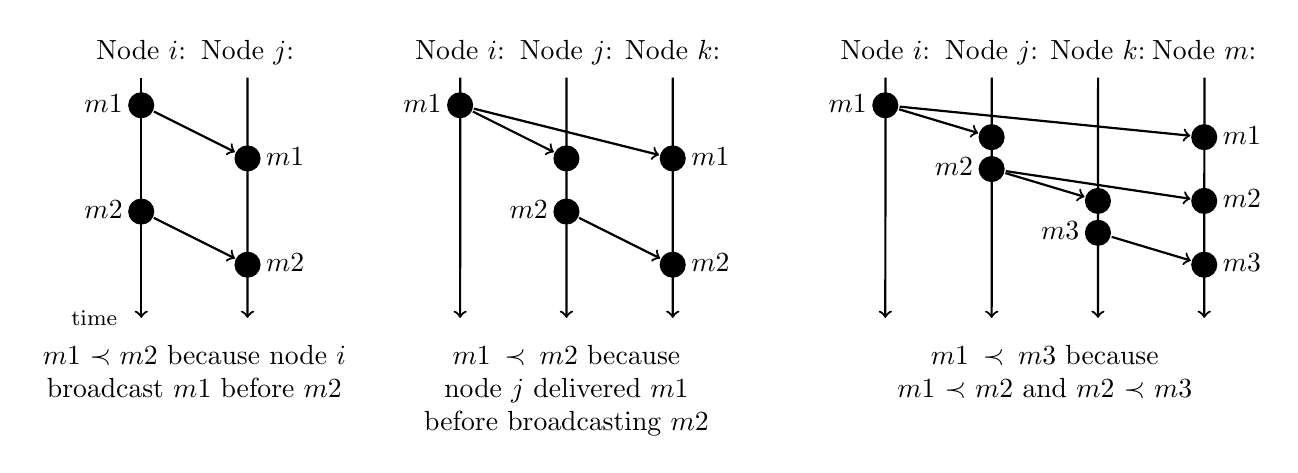
\begin{tikzpicture}[auto,scale=1.35]

\tikzstyle{event}=[circle,fill,minimum size=2pt]
\tikzstyle{label}=[text height=8pt,text depth=3pt]
\tikzstyle{leftlabel}=[label,left=3pt]
\tikzstyle{rightlabel}=[label,right=3pt]
\tikzstyle{every path}=[thick,->]
\tikzstyle{caption}=[text width=4cm,text centered,text height=8pt,below=5pt]

\node [label] (i1name) at (0,2.5) {Node $i$:};
\node [label] (j1name) at (1,2.5) {Node $j$:};
\node [event] (op1send) at (0,2.0) {};
\node [event] (op1recv) at (1,1.5) {};
\node [event] (op2send) at (0,1.0) {};
\node [event] (op2recv) at (1,0.5) {};
\node [leftlabel]  at (0,2.0) {$\isa{m1}$};
\node [rightlabel] at (1,1.5) {$\isa{m1}$};
\node [leftlabel]  at (0,1.0) {$\isa{m2}$};
\node [rightlabel] at (1,0.5) {$\isa{m2}$};
\draw (i1name) -- (0,0) node [left=5pt,at end] {\footnotesize time};
\draw (j1name) -- (1,0);
\draw (op1send) -- (op1recv);
\draw (op2send) -- (op2recv);
\node [caption] at (0.5,0) {
    $\isa{m1} \prec \isa{m2}$
    because node $i$ broadcast $\isa{m1}$ before $\isa{m2}$
};

\node [label] (i2name) at (3,2.5) {Node $i$:};
\node [label] (j2name) at (4,2.5) {Node $j$:};
\node [label] (k2name) at (5,2.5) {Node $k$:};
\node [event] (op3send) at (3,2.0) {};
\node [event] (op3recj) at (4,1.5) {};
\node [event] (op3reck) at (5,1.5) {};
\node [event] (op4send) at (4,1.0) {};
\node [event] (op4reck) at (5,0.5) {};
\node [leftlabel]  at (3,2.0) {$\isa{m1}$};
\node [rightlabel] at (5,1.5) {$\isa{m1}$};
\node [leftlabel]  at (4,1.0) {$\isa{m2}$};
\node [rightlabel] at (5,0.5) {$\isa{m2}$};
\draw (i2name) -- (3,0);
\draw (j2name) -- (4,0);
\draw (k2name) -- (5,0);
\draw (op3send) -- (op3recj);
\draw (op3send) -- (op3reck);
\draw (op4send) -- (op4reck);
\node [caption] at (4.0,0) {
    $\isa{m1} \prec \isa{m2}$
    because node $j$ delivered $\isa{m1}$ before broadcasting $\isa{m2}$
};

\node [label] (i3name) at  (7,2.5) {Node $i$:};
\node [label] (j3name) at  (8,2.5) {Node $j$:};
\node [label] (k3name) at  (9,2.5) {Node $k$:};
\node [label] (m3name) at (10,2.5) {Node $m$:};
\node [event] (op5send) at  (7,2.0) {};
\node [event] (op5recj) at  (8,1.7) {};
\node [event] (op5recm) at (10,1.7) {};
\node [event] (op6send) at  (8,1.4) {};
\node [event] (op6reck) at  (9,1.1) {};
\node [event] (op6recm) at (10,1.1) {};
\node [event] (op7send) at  (9,0.8) {};
\node [event] (op7recm) at (10,0.5) {};
\node [leftlabel]  at  (7,2.0) {$\isa{m1}$};
\node [rightlabel] at (10,1.7) {$\isa{m1}$};
\node [leftlabel]  at  (8,1.4) {$\isa{m2}$};
\node [rightlabel] at (10,1.1) {$\isa{m2}$};
\node [leftlabel]  at  (9,0.8) {$\isa{m3}$};
\node [rightlabel] at (10,0.5) {$\isa{m3}$};
\draw (i3name) -- (7,0);
\draw (j3name) -- (8,0);
\draw (k3name) -- (9,0);
\draw (m3name) -- (10,0);
\draw (op5send) -- (op5recj);
\draw (op5send) -- (op5recm);
\draw (op6send) -- (op6reck);
\draw (op6send) -- (op6recm);
\draw (op7send) -- (op7recm);
\node [caption] at (8.5,0) {
    $\isa{m1} \prec \isa{m3}$ because
    $\isa{m1} \prec \isa{m2}$ and
    $\isa{m2} \prec \isa{m3}$
};

\end{tikzpicture}

\caption{Illustrating the happens-before relation}\label{fig.happens-before}
\end{figure}

Figure~\ref{fig.happens-before} illustrates these three cases, and the formalisation of this
definition appears in Section~\ref{sect.network}.

In practice, the happens-before relationship can be captured using vector timestamps
\cite{Schwarz:1994gl,Fidge:1988tv,Raynal:1996jl}, which are used to implement protocols for causally
ordered delivery \cite{Cachin:2011wt}. As these protocols are widely known and well understood, we
leave them out of scope for this paper.


% Total order broadcast ensures that when nodes broadcast a set of messages to other nodes on the
% network, they are delivered in the same order to all recipients. By contrast, causal ordering is a
% weaker guarantee that allows greater concurrency and thus greater nondeterminism in the network.
% However, it has the advantage that it makes no assumptions about the number of nodes that are
% online.

% TODO happens-before


% There are two families of algorithms for collaborative editing: \emph{operational transformation}
% (OT)~\cite{Ellis:1989ue,Ressel:1996wx,Oster:2006tr,Sun:1998vf,Sun:1998un,Suleiman:1998eu,Nichols:1995fd}
% and \emph{conflict-free replicated datatypes}
% (CRDTs)~\cite{Shapiro:2011wy,Roh:2011dw,Preguica:2009fz,Oster:2006wj,Weiss:2010hx,Nedelec:2013ky,Kleppmann:2016ve}.
% Both allow a document to be modified concurrently on different replicas, with changes applied
% immediately to the local copy, while asynchronously propagating changes to other replicas. The
% goal of these algorithms is to ensure that for all concurrent executions, the replicas converge
% toward the same state without any edits being lost, a property known as \emph{strong eventual
% consistency}~\cite{Shapiro:2011un}.


% CRDTs are a more recent development~\cite{Shapiro:2011un}. While OT is based on transforming
% non-commutative operations so that they have the same effect when reordered, CRDTs define operations
% in a way that makes them commutative by design, making them more amenable to peer-to-peer settings
% in which each node may apply edits in a different order. CRDTs also have attractive performance
% characteristics~\cite{Mehdi:2011ke}.

% TODO Various decentralised algorithms have been proposed and all but one (Oster 2006) have
% subsequently been shown to be incorrect.

\begin{figure}
\centering
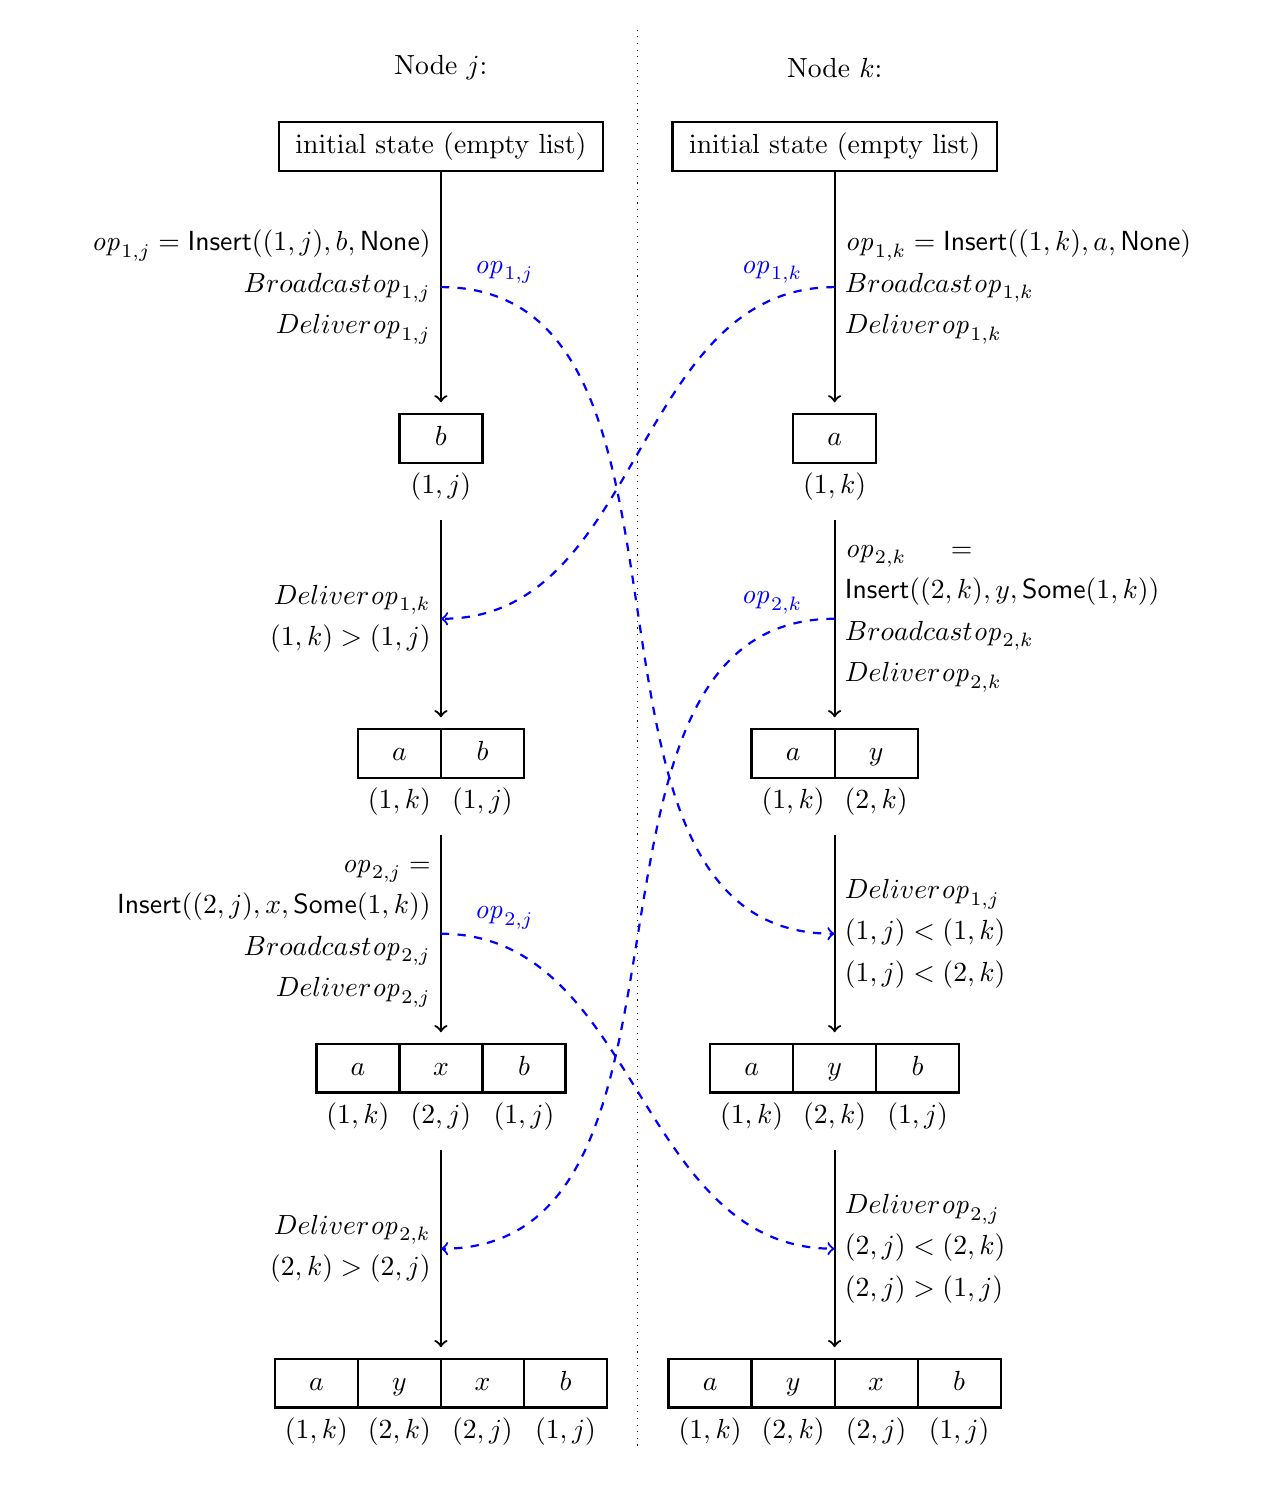
\begin{tikzpicture}[auto,scale=1.0]
\onehalfspacing
\path [draw,dotted] (2.5,-0.5) -- (2.5,17.5);

\tikzstyle{initstate}=[rectangle,draw,inner xsep=6pt,text height=8pt,text depth=3pt]
\tikzstyle{state}=[matrix,column sep={30pt,between origins}]
\tikzstyle{val}=[draw,anchor=base,minimum width=30pt,text height=8pt,text depth=3pt]
\tikzstyle{oid}=[anchor=base]
\tikzstyle{leftevent}=[left,text width=5cm,text ragged left,midway]
\tikzstyle{rightevent}=[right,text width=5cm,text ragged,midway]
\tikzstyle{every path}=[thick,->]

\node (leftR) at (0,17) {Node $j$:};
\node (left1) at (0,16) [initstate] {initial state (empty list)};
\node (left2) at (0,12) [state] {
    \node [val] {$b$};     \\
    \node [oid] {$(1,j)$}; \\
};
\node (left3) at (0,8) [state] {
    \node [val] {$a$};     & \node [val] {$b$};     \\
    \node [oid] {$(1,k)$}; & \node [oid] {$(1,j)$}; \\
};
\node (left4) at (0,4) [state] {
    \node [val] {$a$};     & \node [val] {$x$};     & \node [val] {$b$};     \\
    \node [oid] {$(1,k)$}; & \node [oid] {$(2,j)$}; & \node [oid] {$(1,j)$}; \\
};
\node (left5) at (0,0) [state] {
    \node [val] {$a$};     & \node [val] {$y$};     & \node [val] {$x$};     & \node [val] {$b$};     \\
    \node [oid] {$(1,k)$}; & \node [oid] {$(2,k)$}; & \node [oid] {$(2,j)$}; & \node [oid] {$(1,j)$}; \\
};

\draw (left1) -- (left2) node (send1j) [leftevent] {
    \hfill $\mathit{op}_{1,j} = \mathsf{Insert}((1, j), b, \mathsf{None})$ \\
    \hfill $\text{Broadcast } \mathit{op}_{1,j}$ \\
    \hfill $\text{Deliver } \mathit{op}_{1,j}$ \\
};
\draw (left2) -- (left3) node (recv1k) [leftevent] {
    \hfill $\text{Deliver } \mathit{op}_{1,k}$ \\
    \hfill $(1,k) > (1,j)$ \\
};
\draw (left3) -- (left4) node (send2j) [leftevent] {
    \hfill $\mathit{op}_{2,j} = \mathsf{Insert}((2, j), x, \mathsf{Some}(1,k))$ \\
    \hfill $\text{Broadcast } \mathit{op}_{2,j}$ \\
    \hfill $\text{Deliver } \mathit{op}_{2,j}$ \\
};
\draw (left4) -- (left5) node (recv2k) [leftevent] {
    \hfill $\text{Deliver } \mathit{op}_{2,k}$ \\
    \hfill $(2,k) > (2,j)$ \\
};

\node (rightR) at (5,17) {Node $k$:};
\node (right1) at (5,16) [initstate] {initial state (empty list)};
\node (right2) at (5,12) [state] {
    \node [val] {$a$};     \\
    \node [oid] {$(1,k)$}; \\
};
\node (right3) at (5,8) [state] {
    \node [val] {$a$};     & \node [val] {$y$};     \\
    \node [oid] {$(1,k)$}; & \node [oid] {$(2,k)$}; \\
};
\node (right4) at (5,4) [state] {
    \node [val] {$a$};     & \node [val] {$y$};     & \node [val] {$b$};     \\
    \node [oid] {$(1,k)$}; & \node [oid] {$(2,k)$}; & \node [oid] {$(1,j)$}; \\
};
\node (right5) at (5,0) [state] {
    \node [val] {$a$};     & \node [val] {$y$};     & \node [val] {$x$};     & \node [val] {$b$};     \\
    \node [oid] {$(1,k)$}; & \node [oid] {$(2,k)$}; & \node [oid] {$(2,j)$}; & \node [oid] {$(1,j)$}; \\
};

\draw (right1) -- (right2) node (send1k) [rightevent] {
    $\mathit{op}_{1,k} = \mathsf{Insert}((1, k), a, \mathsf{None})$ \\
    $\text{Broadcast } \mathit{op}_{1,k}$ \\
    $\text{Deliver } \mathit{op}_{1,k}$ \\
};
\draw (right2) -- (right3) node (send2k) [rightevent] {
    $\mathit{op}_{2,k} = \mathsf{Insert}((2, k), y, \mathsf{Some}(1, k))$ \\
    $\text{Broadcast } \mathit{op}_{2,k}$ \\
    $\text{Deliver } \mathit{op}_{2,k}$ \\
};
\draw (right3) -- (right4) node (recv1j) [rightevent] {
    $\text{Deliver } \mathit{op}_{1,j}$ \\
    $(1,j) < (1,k)$ \\
    $(1,j) < (2,k)$ \\
};
\draw (right4) -- (right5) node (recv2j) [rightevent] {
    $\text{Deliver } \mathit{op}_{2,j}$ \\
    $(2,j) < (2,k)$ \\
    $(2,j) > (1,j)$ \\
};

\begin{scope}[dashed,blue]
    \tikzstyle{every node}=[text centered]
    \draw (send1j.east) to [out=0,in=180] (recv1j.west);
    \draw (send2j.east) to [out=0,in=180] (recv2j.west);
    \draw (send1k.west) to [out=180,in=0] (recv1k.east);
    \draw (send2k.west) to [out=180,in=0] (recv2k.east);
    \node at (0.8,14.4) {$\mathit{op}_{1,j}$};
    \node at (0.8, 6.2) {$\mathit{op}_{2,j}$};
    \node at (4.2,14.4) {$\mathit{op}_{1,k}$};
    \node at (4.2,10.2) {$\mathit{op}_{2,k}$};
\end{scope}
\end{tikzpicture}

\caption{RGA example}\label{fig.two-lists}
\end{figure}


\begin{figure}[t]
  \raggedright
  \begin{isabellebody}
\isanewline
\isacommand{theorem}\isamarkupfalse%
\ \ convergence{\isacharcolon}\isanewline
\ \ \isakeyword{assumes}\ {\isachardoublequoteopen}set\ xs\ {\isacharequal}\ set\ ys{\isachardoublequoteclose}\isanewline
\ \ \ \ \ \ \ \ \ \ {\isachardoublequoteopen}concurrent{\isacharunderscore}ops{\isacharunderscore}commute\ xs{\isachardoublequoteclose}\isanewline
\ \ \ \ \ \ \ \ \ \ {\isachardoublequoteopen}concurrent{\isacharunderscore}ops{\isacharunderscore}commute\ ys{\isachardoublequoteclose}\isanewline
\ \ \ \ \ \ \ \ \ \ {\isachardoublequoteopen}distinct\ xs{\isachardoublequoteclose}\isanewline
\ \ \ \ \ \ \ \ \ \ {\isachardoublequoteopen}distinct\ ys{\isachardoublequoteclose}\isanewline
\ \ \ \ \ \ \ \ \ \ {\isachardoublequoteopen}hb{\isacharunderscore}consistent\ xs{\isachardoublequoteclose}\isanewline
\ \ \ \ \ \ \ \ \ \ {\isachardoublequoteopen}hb{\isacharunderscore}consistent\ ys{\isachardoublequoteclose}\isanewline
\ \ \isakeyword{shows}\ \ \ {\isachardoublequoteopen}apply{\isacharunderscore}operations\ xs\ {\isacharequal}\ apply{\isacharunderscore}operations\ ys{\isachardoublequoteclose}\isanewline
%
\isacommand{using}\isamarkupfalse%
\ assms\ \isacommand{proof}\isamarkupfalse%
{\isacharparenleft}induction\ xs\ arbitrary{\isacharcolon}\ ys\ rule{\isacharcolon}\ rev{\isacharunderscore}induct{\isacharcomma}\ simp{\isacharparenright}\isanewline
\ \ \isacommand{case}\isamarkupfalse%
\ assms{\isacharcolon}\ {\isacharparenleft}snoc\ x\ xs{\isacharparenright}\isanewline
\ \ \isacommand{then}\isamarkupfalse%
\ \isacommand{obtain}\isamarkupfalse%
\ prefix\ suffix\ \isakeyword{where}\ ys{\isacharunderscore}split{\isacharcolon}\ {\isachardoublequoteopen}ys\ {\isacharequal}\ prefix\ {\isacharat}\ x\ {\isacharhash}\ suffix\ {\isasymand}\ concurrent{\isacharunderscore}set\ x\ suffix{\isachardoublequoteclose}\isanewline
\ \ \ \ \isacommand{using}\isamarkupfalse%
\ hb{\isacharunderscore}consistent{\isacharunderscore}prefix{\isacharunderscore}suffix{\isacharunderscore}exists\ \isacommand{by}\isamarkupfalse%
\ fastforce\isanewline
\ \ \isacommand{moreover}\isamarkupfalse%
\ \isacommand{hence}\isamarkupfalse%
\ {\isacharasterisk}{\isacharcolon}\ {\isachardoublequoteopen}distinct\ {\isacharparenleft}prefix\ {\isacharat}\ suffix{\isacharparenright}{\isachardoublequoteclose}\ {\isachardoublequoteopen}hb{\isacharunderscore}consistent\ xs{\isachardoublequoteclose}\isanewline
\ \ \ \ \isacommand{using}\isamarkupfalse%
\ assms\ \isacommand{by}\isamarkupfalse%
\ auto\isanewline
\ \ \isacommand{moreover}\isamarkupfalse%
\ \isacommand{{\isacharbraceleft}}\isamarkupfalse%
\isanewline
\ \ \ \ \isacommand{have}\isamarkupfalse%
\ {\isachardoublequoteopen}hb{\isacharunderscore}consistent\ prefix{\isachardoublequoteclose}\ {\isachardoublequoteopen}hb{\isacharunderscore}consistent\ suffix{\isachardoublequoteclose}\isanewline
\ \ \ \ \ \ \isacommand{using}\isamarkupfalse%
\ ys{\isacharunderscore}split\ assms\ hb{\isacharunderscore}consistent{\isacharunderscore}append{\isacharunderscore}D{\isadigit{2}}\ hb{\isacharunderscore}consistent{\isacharunderscore}append{\isacharunderscore}elim{\isacharunderscore}ConsD\ \isacommand{by}\isamarkupfalse%
\ blast{\isacharplus}\isanewline
\ \ \ \ \isacommand{hence}\isamarkupfalse%
\ {\isachardoublequoteopen}hb{\isacharunderscore}consistent\ {\isacharparenleft}prefix\ {\isacharat}\ suffix{\isacharparenright}{\isachardoublequoteclose}\isanewline
\ \ \ \ \ \ \isacommand{by}\isamarkupfalse%
\ {\isacharparenleft}metis\ assms{\isacharparenleft}{\isadigit{8}}{\isacharparenright}\ hb{\isacharunderscore}consistent{\isacharunderscore}append\ hb{\isacharunderscore}consistent{\isacharunderscore}append{\isacharunderscore}porder\ list{\isachardot}set{\isacharunderscore}intros{\isacharparenleft}{\isadigit{2}}{\isacharparenright}\ ys{\isacharunderscore}split{\isacharparenright}\isanewline
\ \ \isacommand{{\isacharbraceright}}\isamarkupfalse%
\isanewline
\ \ \isacommand{moreover}\isamarkupfalse%
\ \isacommand{have}\isamarkupfalse%
\ {\isacharasterisk}{\isacharasterisk}{\isacharcolon}\ {\isachardoublequoteopen}concurrent{\isacharunderscore}ops{\isacharunderscore}commute\ {\isacharparenleft}prefix\ {\isacharat}\ suffix\ {\isacharat}\ {\isacharbrackleft}x{\isacharbrackright}{\isacharparenright}{\isachardoublequoteclose}\isanewline
\ \ \ \ \isacommand{using}\isamarkupfalse%
\ assms\ ys{\isacharunderscore}split\ \isacommand{by}\isamarkupfalse%
\ {\isacharparenleft}clarsimp\ simp{\isacharcolon}\ concurrent{\isacharunderscore}ops{\isacharunderscore}commute{\isacharunderscore}def{\isacharparenright}\isanewline
\ \ \isacommand{moreover}\isamarkupfalse%
\ \isacommand{hence}\isamarkupfalse%
\ {\isachardoublequoteopen}concurrent{\isacharunderscore}ops{\isacharunderscore}commute\ {\isacharparenleft}prefix\ {\isacharat}\ suffix{\isacharparenright}{\isachardoublequoteclose}\isanewline
\ \ \ \ \isacommand{by}\isamarkupfalse%
\ {\isacharparenleft}force\ simp\ del{\isacharcolon}\ append{\isacharunderscore}assoc\ simp\ add{\isacharcolon}\ append{\isacharunderscore}assoc{\isacharbrackleft}symmetric{\isacharbrackright}{\isacharparenright}\isanewline
\ \ \isacommand{ultimately}\isamarkupfalse%
\ \isacommand{have}\isamarkupfalse%
\ {\isachardoublequoteopen}apply{\isacharunderscore}operations\ xs\ {\isacharequal}\ apply{\isacharunderscore}operations\ {\isacharparenleft}prefix{\isacharat}suffix{\isacharparenright}{\isachardoublequoteclose}\isanewline
\ \ \ \ \isacommand{using}\isamarkupfalse%
\ assms\ \isacommand{by}\isamarkupfalse%
\ simp\ {\isacharparenleft}metis\ Diff{\isacharunderscore}insert{\isacharunderscore}absorb\ Un{\isacharunderscore}iff\ {\isacharasterisk}\ concurrent{\isacharunderscore}ops{\isacharunderscore}commute{\isacharunderscore}appendD\ set{\isacharunderscore}append{\isacharparenright}\isanewline
\ \ \isacommand{moreover}\isamarkupfalse%
\ \isacommand{have}\isamarkupfalse%
\ {\isachardoublequoteopen}apply{\isacharunderscore}operations\ {\isacharparenleft}prefix{\isacharat}suffix\ {\isacharat}\ {\isacharbrackleft}x{\isacharbrackright}{\isacharparenright}\ {\isacharequal}\ apply{\isacharunderscore}operations\ {\isacharparenleft}prefix{\isacharat}x\ {\isacharhash}\ suffix{\isacharparenright}{\isachardoublequoteclose}\isanewline
\ \ \ \ \isacommand{using}\isamarkupfalse%
\ ys{\isacharunderscore}split\ assms\ {\isacharasterisk}{\isacharasterisk}\ concurrent{\isacharunderscore}ops{\isacharunderscore}commute{\isacharunderscore}concurrent{\isacharunderscore}set\ \isacommand{by}\isamarkupfalse%
\ force\isanewline
\ \ \isacommand{ultimately}\isamarkupfalse%
\ \isacommand{show}\isamarkupfalse%
\ {\isacharquery}case\isanewline
\ \ \ \ \isacommand{using}\isamarkupfalse%
\ ys{\isacharunderscore}split\ \isacommand{by}\isamarkupfalse%
\ {\isacharparenleft}force\ simp{\isacharcolon}\ append{\isacharunderscore}assoc{\isacharbrackleft}symmetric{\isacharbrackright}\ simp\ del{\isacharcolon}\ append{\isacharunderscore}assoc{\isacharparenright}\isanewline
\isacommand{qed}\isamarkupfalse%
  \end{isabellebody}
  \caption{Proof of convergence theorem in Isar.}
  \label{fig.convergence}
\end{figure}


\end{document}
